\documentclass[12pt]{article}

\usepackage{fancyhdr}
\usepackage{fullpage}
\usepackage{amsmath}
\usepackage{amsbsy}
\usepackage{amssymb}
\usepackage{amscd}
\usepackage{amsfonts}
\usepackage{amsthm}
\usepackage{supertabular}
\usepackage{graphicx}
\usepackage{verbatim}
\usepackage{epsfig}
\usepackage{xspace}
\usepackage{euscript}
\usepackage{alltt}
\usepackage{boxedminipage}
\usepackage{float}
\usepackage{times}
\usepackage{epic}
\usepackage{eepic}
\usepackage{ifthen}
\usepackage{algorithm}
\usepackage{booktabs}
\usepackage{multirow}
\usepackage{cancel}
%\usepackage[colorlinks]{hyperref}
\usepackage[numbers,sort&compress]{natbib}
\usepackage[FIGBOTCAP,TABTOPCAP,bf,tight]{subfigure}



\usepackage[T1]{fontenc}
\usepackage{ae,aecompl}

\newcommand{\mbs}[1]{\boldsymbol{#1}}
\newcommand{\mbb}[1]{\mathbb{#1}}
\newcommand{\mbf}[1]{\mathbf{#1}}
\newcommand{\mbc}[1]{\boldsymbol{\mathcal{#1}}}

\newtheorem*{proposition}{Proposition}

\def\ljump{\lbrack\!\lbrack} \def\rjump{\rbrack\!\rbrack}

\def\bA{{\mbs{A}}} \def\bB{{\mbs{B}}} \def\bC{{\mbs{C}}}
\def\bD{{\mbs{D}}} \def\bE{{\mbs{E}}} \def\bF{{\mbs{F}}}
\def\bG{{\mbs{G}}} \def\bH{{\mbs{H}}} \def\bI{{\mbs{I}}}
\def\bJ{{\mbs{J}}} \def\bK{{\mbs{K}}} \def\bL{{\mbs{L}}}
\def\bM{{\mbs{M}}} \def\bN{{\mbs{N}}} \def\bO{{\mbs{O}}}
\def\bP{{\mbs{P}}} \def\bQ{{\mbs{Q}}} \def\bR{{\mbs{R}}}
\def\bS{{\mbs{S}}} \def\bT{{\mbs{T}}} \def\bU{{\mbs{U}}}
\def\bV{{\mbs{V}}} \def\bW{{\mbs{W}}} \def\bX{{\mbs{X}}}
\def\bY{{\mbs{Y}}} \def\bZ{{\mbs{Z}}}

\def\ba{{\mbs{a}}} \def\bb{{\mbs{b}}} \def\bc{{\mbs{c}}}
\def\bd{{\mbs{d}}} \def\be{{\mbs{e}}} \def\fb{{\mbs{f}}}
\def\bg{{\mbs{g}}} \def\bh{{\mbs{h}}} \def\bi{{\mbs{i}}}
\def\bj{{\mbs{j}}} \def\bk{{\mbs{k}}} \def\bl{{\mbs{l}}}
\def\bm{{\mbs{m}}} \def\bn{{\mbs{n}}} \def\bo{{\mbs{o}}}
\def\bp{{\mbs{p}}} \def\bq{{\mbs{q}}} \def\br{{\mbs{r}}}
\def\bs{{\mbs{s}}} \def\bt{{\mbs{t}}} \def\bu{{\mbs{u}}}
\def\bv{{\mbs{v}}} \def\bw{{\mbs{w}}} \def\bx{{\mbs{x}}}
\def\by{{\mbs{y}}} \def\bz{{\mbs{z}}}

\def\balpha{{\mbs{\alpha}}}
\def\bbeta{{\mbs{\beta}}}
\def\bgamma{{\mbs{\gamma}}}
\def\bdelta{{\mbs{\delta}}}
\def\bepsilon{{\mbs{\epsilon}}}
\def\bvarepsilon{{\mbs{\varepsilon}}}
\def\bzeta{{\mbs{\zeta}}}
\def\beeta{{\mbs{\eta}}}
\def\btheta{{\mbs{\theta}}}
\def\bvartheta{{\mbs{\vartheta}}}
\def\bgamma{{\mbs{\gamma}}}
\def\bkappa{{\mbs{\kappa}}}
\def\blambda{{\mbs{\lambda}}}
\def\bmu{{\mbs{\mu}}}
\def\bnu{{\mbs{\nu}}}
\def\bxi{{\mbs{\xi}}}
\def\bomicron{{\mbs{o}}}
\def\bpi{{\mbs{\pi}}}
\def\bvarpi{{\mbs{\varpi}}}
\def\brho{{\mbs{\rho}}}
\def\bvarrho{{\mbs{\varrho}}}
\def\bsigma{{\mbs{\sigma}}}
\def\bvarsigma{{\mbs{\varsigma}}}
\def\btau{{\mbs{\tau}}}
\def\bupsilon{{\mbs{\upsilon}}}
\def\bphi{{\mbs{\phi}}}
\def\bvarphi{{\mbs{\varphi}}}
\def\bchi{{\mbs{\chi}}}
\def\bpsi{{\mbs{\psi}}}
\def\bomega{{\mbs{\omega}}}

\def\bGamma{{\mbs{\Gamma}}}
\def\bDelta{{\mbs{\Delta}}}
\def\bTheta{{\mbs{\Theta}}}
\def\bLambda{{\mbs{\Lambda}}}
\def\bXi{{\mbs{\Xi}}}
\def\bPi{{\mbs{\Pi}}}
\def\bSigma{{\mbs{\Sigma}}}
\def\bUpsilon{{\mbs{\Upsilon}}}
\def\bPhi{{\mbs{\Phi}}}
\def\bPsi{{\mbs{\Psi}}}
\def\bOmega{{\mbs{\Omega}}}

\def\dt{{\triangle t}}

\DeclareMathOperator{\tr}{tr}

\DeclareMathOperator{\divrg}{div}
\DeclareMathOperator{\grad}{grad}
\DeclareMathOperator{\curl}{curl}

\DeclareMathOperator{\Div}{Div}
\DeclareMathOperator{\Grad}{Grad}
\DeclareMathOperator{\Curl}{Curl}

\DeclareMathOperator{\dev}{dev}
\DeclareMathOperator{\vol}{vol}
\DeclareMathOperator{\Dev}{Dev}
\DeclareMathOperator{\Vol}{Vol}

\makeatletter \@addtoreset{figure}{section}
\def\thefigure{\thesection.\@arabic\c@figure} \def\fps@figure{h, t}
\@addtoreset{equation}{section}
\def\theequation{\thesection.\arabic{equation}} \makeatother


\begin{document}

\setlength{\headheight}{15pt}
\headsep = 4pt
\pagestyle{fancyplain}

\lhead
[\fancyplain{}{\emph{A.Mota, W.Sun, J.Ostien, J.Foulk, K.Long}}]
{\fancyplain{}{\emph{A.Mota, W.Sun, J.Ostien, J.Foulk, K.Long}}}

\rhead
[\fancyplain{} {\emph{Transfer Operator for Internal Variables}}]
{\fancyplain{} {\emph{Transfer Operator for Internal Variables}}}

%Remove this in final version
\cfoot
[\fancyplain{}{\bf{DRAFT of \today}}]
{\fancyplain{}{\bf{DRAFT of \today}}}

\title{A Variational Transfer Operator for Mapping of Internal
Variables}

\author{
  \Large
  Alejandro~Mota$^1$\thanks{Email: amota@sandia.gov},
  WaiChing~Sun$^1$,
  Jakob~T.~Ostien$^1$,
  \\
  \Large
  James~W.~Foulk {III}$^1$
  Kevin~N.~Long$^2$,
  \\
  \\
  $^1$Mechanics of Materials Department\\
  Sandia National Laboratories\\
  Livermore CA 94550, USA\\
  \\
  $^2$Solid Mechanics Department\\
  Sandia National Laboratories\\
  Albuquerque NM 87185, USA\\
}

\date{\today}

\maketitle

\begin{abstract}

  A mapping procedure for the transfer of internal variables from one finite
  element mesh (\emph{source}) to another (\emph{target}) is proposed. The
  objective is to perform the transfer with minimum error and at the same time
  guarantee that the mapped variables remain in their admissible spaces.

  The minimization of the error is achieved by a three-field finite element
  formulation. The fields in the formulation are the deformation mapping, the
  \emph{target} (mapped) internal variables and a Lagrange multiplier that
  enforces the equality between the \emph{source} (original) and target internal
  variables. This formulation leads to a transfer operator that is an $L_2$
  projection that minimizes the distance between the source and target internal
  variables as measured in the $L_2$ norm of the internal variable space.

  To ensure that the target internal variables remain in their original space,
  their interpolation is performed by recourse to Lie groups, which allow for
  direct polynomial interpolation of the corresponding Lie algebras by means of
  the logarithmic map. Once the Lie algebras are interpolated, the mapped
  variables are recovered by the exponential map, thus guaranteeing that they
  remain in the appropriate space.

\end{abstract}

\section{Introduction}

The transfer of field data from one finite element mesh to another is a need
that arises frequently within the context of mesh adaption in the finite element
method \citep{Ortiz.Quigley:1991, Peric.etal:1996,
  Radovitzky.Ortiz:1999, Rashid:2002, Jiao.Heath:2004, Orlando.Peric:2004,
  Bucher.etal:2007}. Field data that are available
at the nodes may be directly mapped by using the interpolation functions
corresponding to each field. The situation is more complicated, however, in
simulations that carry state information in internal variables, as these are
normally available only at integration points.

Different methods have been devised to map internal variables from one mesh to
another. \citet{Ortiz.Quigley:1991} propose transfer operators based on a
three-field Hu-Washizu formulation. By choosing discontinuous interpolation
functions for the deformation gradient and first Piola-Kirchhoff stress fields,
the authors derive transfer operators that are local to each element.
\citet{Radovitzky.Ortiz:1999} use a transfer operator which reduces to
extrapolation of the internal variables from the integration points in the
source mesh to the integration points in the target mesh.  \citet{Rashid:2002}
introduces a method that assumes constant values for the internal variables
within the cells of a Voronoi tessellation based on the integration points of
the original mesh. These values are then transferred to the final mesh using
another Voronoi tessellation and an algorithm for finding the intersecting
volumes of the cells corresponding to the source and target meshes.
\citet{Jiao.Heath:2004} propose a technique for transferring information in
surface meshes based on a third mesh that they term common refinement. This mesh
is conformal to both the source and target surface meshes. The authors then
proceed to define an $L_2$ minimization between the source and target internal
variable fields for the transfer. They also note the desirable properties of the
$L_2$ minimization for mapping, such as that it requires solving a linear system
of equations with a corresponding matrix that is positive-definite and sparse.
\citet{Bucher.etal:2007} derive transfer operators that extrapolate the internal
variables at integration points to nodes in the source mesh using serendipity
interpolation functions.

It is common for finite deformation constitutive models to be endowed with
internal variables that do not belong to linear spaces. Nevertheless, a problem
that is prevalent to the mapping procedures hitherto described is that they
transfer internal variables with the addition operator, typically via Lagrange
interpolation. This operator, however, may not be admissible in the spaces in
which these variables exist, and as a consequence such procedures do not, in
general, guarantee that transferred internal variables remain in their
appropriate spaces. For example, a scalar isotropic damage parameter might be
extrapolated outside of its admissible range, $[0,1)$.

We propose a three-field finite element formulation as a method for transferring
internal variables from one finite element mesh to another. The additional
fields in the formulation are the target field of internal variables and a
Lagrange multiplier that enforces the equality between the source and target
internal variables. The Lagrange multiplier is subsequently identified as the
corresponding conjugate thermodynamic force. The formulation leads to
expressions for the target internal variables that are $L_2$ projections of the
source internal variables onto the space spanned by the interpolation functions
selected for the extra fields. By using a variational approach, the distance
between the source and target internal variable fields is minimized in the $L_2$
norm of their space, and thus the projection is orthogonal and the corresponding
operator is self-adjoint. The matrices that results from the operator are
symmetric positive definite, sparse and of narrow band.

Next it is shown that for a set of common internal variables, the Lie algebras
corresponding to these variables lie in linear spaces and are therefore suitable
for polynomial interpolation.  The proposed mapping scheme preserves the
constraints imposed on the internal variables as long as they belong to a Lie
group. We adhere to the classical definition of internal variables as fields
that are endowed with their own evolution equations as to eliminate the explicit
dependence of the stored energy function from the history of deformation
\citep{Muschik:2001, Antman:2005}. Thus, the proposed variational principle
states that thermodynamic forces conjugate to the internal variables (such as
stresses) are not mapped, but are computed instead based on the target internal
variables, thereby satisfying their own constraints (such as that stresses be
within the elastic domain) and balance laws.

Assuming that internal variables belong to Lie groups, the corresponding Lie
algebras may be obtained using the logarithmic map. Upon interpolation in the
Lie algebra, the internal variable of interest is recovered by using the
exponential map \citep{Marsden.Ratiu:1999, Sepanski:2007,
Kosmann-Schwarzbach:2009,
  Gallier:2011}. The computation of the logarithmic map may be
effected by using explicit formulae (if the eigenvalues are readily available)
\citep{Jog:2008} or the inverse scaling and squaring algorithm with Pad\'e
approximants \citep{Cheng.etal:2001,
  Davies.Higham:2003}.  A fast and accurate method for the computation
of the exponential map is provided by the scaling and squaring algorithm with
Pad\'e approximants \citep{Higham:2001,Higham:2005}. Most fields of interest,
however, admit a polar decomposition and thus it proves convenient to effect the
interpolation of these fields by interpolating separately their rotational and
stretch components. An added benefit of this method is that the computation of
logarithmic maps for these components is relatively straightforward.

Finally, the $L_2$ projection and Lie algebra interpolation are applied first
separately and then concurrently to selected numerical examples to demonstrate
their effect on the mapping of internal variables.


\section{Finite Element Formulation}
\label{sec:FE-formulation}

Consider a body $B\subset\mbb{R}^3$ undergoing a motion described by
the mapping $\bx = \bvarphi(\bX, t): B\times[t_1, t_2]\rightarrow
\mbb{R}^3$, with the deformation gradient defined by $\bF := \Grad
\bvarphi$.

Assume that the boundary $\partial B$, with unit normal $\bN$, is the
union of a displacement boundary $\partial_{\varphi} B$, where
boundary displacements $\bchi : \partial_{\varphi} B\times[t_1,
t_2]\rightarrow \mbb{R}^3$ are prescribed, and a traction boundary
$\partial_T B$, where tractions $\bT: \partial_T B \times[t_1,
t_2]\rightarrow \mbb{R}^3$ are applied $(\partial_{\varphi} B \cap
\partial_T B = \emptyset)$. Let also $\rho_0 \bB: B \times [t_1,
t_2]\rightarrow \mbb{R}^3$ be the body force, with $\rho_0$ the mass
density in the reference configuration.  Furthermore, for every $t \in
[t_1, t_2]$ introduce the energy functional
\begin{equation}\label{eq:energy}
  \Phi_0[ \bvarphi ] :=
  \int_B W(\bF, \bz) \ dV
  -
  \int_B \rho_0 \bB \cdot \bvarphi \ dV
  -
  \int_{\partial_T B} \bT \cdot \bvarphi \ dS,
\end{equation}
in which $W(\bF, \bz)$ is the Helmholtz free-energy density and $\bz$
is a collection of internal variables. This functional is modified by
introducing a constraint as
\begin{equation}\label{eq:energy-constraint}
  \Phi[ \bvarphi, \bar{\bz}, \bar{\by} ] :=
  \int_B W(\bF, \bar{\bz}) \ dV
  +
  \int_B \bar{\by} \cdot (\bar{\bz} - \bz) \ dV
  -
  \int_B \rho_0 \bB \cdot \bvarphi \ dV
  -
  \int_{\partial_T B} \bT \cdot \bvarphi \ dS,
\end{equation}
in which $\bar{\bz}$ is the field of mapped internal variables that is
constrained to be equal to $\bz$ by means of the Lagrange multiplier
$\bar{\by}$. Although the Helmholtz free-energy density $W$ is now
evaluated using $\bar{\bz}$ instead of $\bz$, the functionals in
\eqref{eq:energy} and \eqref{eq:energy-constraint} are equivalent at
this stage due to this constraint.

Assume that $\bvarphi \in U := (W^1_2(B))^3$, $\bar{\bz}, \bar{\by}
\in V := (W^1_2(B))^q$, in which $W^1_2(B)$ is the Sobolev space of
square-integrable functions with square-integrable first derivatives,
and $q$ is the number of parameters used to represent the internal
variables. The functional \eqref{eq:energy-constraint} is optimized
by applying variations with respect to the independent fields
$\bvarphi$, $\bar{\bz}$ and $\bar{\by}$. Define test functions
corresponding to these fields as $\beeta \in U$, $\bzeta, \bxi \in V$,
with $\beeta = \mathbf{0}$ on $\partial_{\varphi}B$. The variations
follow as
\begin{align}\label{eq:variations-phi}
  D\Phi[ \bvarphi, \bar{\bz}, \bar{\by} ](\beeta)
  & =
  \int_B \bP : \Grad \beeta \ dV - \int_B \rho_0 \bB \cdot \beeta \ dV
  -
  \int_{\partial_T B} \bT \cdot \beeta \ dS = 0,
  \\
  D\Phi[ \bvarphi, \bar{\bz}, \bar{\by} ](\bzeta)
  & =
  \int_B (\bar{\by} - \by) \cdot \bzeta \ dV = 0,
  \label{eq:variations-y}
  \\
  D\Phi[ \bvarphi, \bar{\bz}, \bar{\by} ](\bxi)
  & =
  \int_B (\bar{\bz} - \bz) \cdot \bxi \ dV = 0,
  \label{eq:variations-z}
\end{align}
where $\bP := \partial W / \partial \bF$ is the first Piola-Kirchhoff
stress and $\by := - \partial W / \partial \bar{\bz}$ is the
thermodynamic force conjugate to $\bar{\bz}$. The corresponding
Euler-Lagrange equations are
\begin{gather}
  \Div \bP + \rho_0 \bB = \mathbf{0} \text{ in } B, \quad
  \bP \bN = \bT \text{ on } \partial_T B, \label{eq:equilibrium}
  \\
  \bar{\by} = \by \text{ in } B,
  \\
  \bar{\bz} = \bz \text{ in } B,
\end{gather}
as expected. Note that the equilibrium condition \eqref{eq:equilibrium}
is evaluated using the mapped internal variable field $\bar{\bz}$, and
therefore equlibrium and constitutive constraints are satisfied using
this field. Next, introduce discretizations for the fields and test
functions as
\begin{align}
  \bvarphi_h(\bX) := N_a(\bX) \bvarphi_a \in U_h,
  & \quad
  \beeta_h(\bX) := N_b(\bX) \beeta_b \in U_h,
  \\
  \bar{\bz}_h(\bX) := \lambda_\alpha(\bX) \bar{\bz}_\alpha \in V_h,
  & \quad
  \bzeta_h(\bX) := \lambda_\beta(\bX) \bzeta_\beta \in V_h,
  \\
  \bar{\by}_h(\bX) := \lambda_\alpha(\bX) \bar{\by}_\alpha \in V_h,
  & \quad
  \bxi_h(\bX) := \lambda_\beta(\bX) \bxi_\beta \in V_h,
\end{align}
where $N_a$ and $N_b$ are interpolation functions for $\bvarphi$ and
$\beeta$, $\lambda_\alpha$ and $\lambda_\beta$ are interpolation
functions for $(\bar{\bz}, \bar{\by})$ and $(\bzeta, \bxi)$, and
$(a,b) \in [1 \ldots N]$ and $(\alpha, \beta) \in [1 \ldots M]$, in
which $N$ is the number of nodes for $\bvarphi$, $M$ is the number of
nodes for $\bar{\bz}$ and $\bar{\by}$ respectively, and $U_h \subset
U$, and $V_h \subset V$. Introducing these discretizations
into the variational statements
\eqref{eq:variations-phi}-\eqref{eq:variations-z} gives
\begin{gather}
  \int_B \bP \cdot \Grad N_a \ dV
  -
  \int_B \rho_0 \bB N_a \ dV
  -
  \int_{\partial_T B} \bT N_a \ dS
  =
  \mathbf{0}, \label{eq:discrete-equilibrium}
  \\
  \bar{\by}_h
  =
  \lambda_\alpha
  \left(
  \int_B \lambda_\alpha \lambda_\beta \bI \ dV
  \right)^{-1}
  \int_B \lambda_\beta \by \ dV, \label{eq:projection-y}
  \\
  \bar{\bz}_h
  =
  \lambda_\alpha
  \left(
  \int_B \lambda_\alpha \lambda_\beta \bI \ dV
  \right)^{-1}
  \int_B \lambda_\beta \bz \ dV, \label{eq:projection-z}
\end{gather}
which are the discrete statements of equilibrium, the discrete
thermodynamic forces and internal variables, respectively, and with
$\bI$ being the $q \times q$ identity. Note that
\eqref{eq:projection-y} and \eqref{eq:projection-z} are projections of
the fields $\by$ and $\bz$ onto $V_h$, as by definition
$\lambda_\alpha$ and $\lambda_\beta$ form a basis for this space.
Effective computation of the integrals in these expressions readily
suggests using interpolation functions $\lambda_\alpha$ and
$\lambda_\beta$ that are of the same order or less than $N_a$ and
$N_b$. This allows the use of the same integration scheme for
\eqref{eq:projection-y} and \eqref{eq:projection-z} as for
\eqref{eq:discrete-equilibrium}, ensuring that the projections will be
fully integrated (provided that full integration is used for the
equilibrium statement as well) using the same integration points (thus
avoiding any unnecessary transfer of variables at this
stage). Furthermore, if the interpolation functions $\lambda_\alpha$
and $\lambda_\beta$ are discontinuous across element boundaries, the
projection \eqref{eq:projection-z} reduces to extrapolation of values
from integration points to nodes (cf. \citet{Ortiz.Quigley:1991,
  Radovitzky.Ortiz:1999}).  Next we show that the projection is
optimal.

\begin{proposition}
  The projection defined by \eqref{eq:projection-z} is orthogonal with
  respect to $V_h$ and therefore the distance between source and
  target fields is minimal in the $L_2$ norm of $V$.
\end{proposition}

\begin{proof}
Define the inner product in $V$ as
\begin{equation}
  (\bu, \bv) := \int_B \bu \cdot \bv \ dV,
  \quad
  \forall \, \bu, \bv \in V,
  \label{eq:inner-product}
\end{equation}
and the corresponding $L_2$ norm as
\begin{equation}
  ||\bu|| :=
  \left( \int_B \bu \cdot \bu \ dV \right)^{\frac{1}{2}}
  \ge 0,
  \quad
  \forall \, \bu \in V.
  \label{eq:norm}
\end{equation}

We follow the approach outlined by \citet{Brenner.Scott:2002}. The
variational statement \eqref{eq:variations-z} may be written after
discretization as
\begin{equation}
  \int_B (\bar{\bz}_h - \bz) \cdot \bxi_h \ dV = 0
  \label{eq:variations-z-discrete}
\end{equation}
where $\bz \in V$ and $\bar{\bz}_h, \bxi_h \in V_h$. Using
the inner product notation introduced in \eqref{eq:inner-product} this
discrete statement takes the form
\begin{equation}
  (\bar{\bz}_h - \bz, \bxi_h) = 0, \quad \forall \bxi_h \in V_h
  \label{eq:orthogonality}
\end{equation}
which shows the fundamental orthogonality relation between the
projection error $\bar{\bz}_h - \bz$ and the space $V_h$,
therefore proving that \eqref{eq:projection-z} is an orthogonal
projection. Introduce the Cauchy-Schwarz inequality
\begin{equation}
  (\bu, \bv) \le ||\bu|| ||\bv||, \quad \forall \bu, \bv \in V,
  \label{eq:Cauchy-Schwarz}
\end{equation}
then for any $\bu_h \in V_h$
\begin{align}
  ||\bar{\bz}_h - \bz||^2 & = (\bar{\bz}_h - \bz, \bar{\bz}_h - \bz)
  \\
  & = (\bar{\bz}_h - \bz, \bu_h - \bz) +
  (\bar{\bz}_h - \bz, \bar{\bz}_h - \bu_h)
  \\
  & = (\bar{\bz}_h - \bz, \bu_h - \bz) \quad
  \text{from \eqref{eq:orthogonality} with
    $\bxi_h = \bar{\bz}_h - \bu_h$}
  \\
  & \le ||\bar{\bz}_h - \bz|| ||\bu_h - \bz|| \quad
  \text{from \eqref{eq:Cauchy-Schwarz}}.
  \label{eq:inequality}
\end{align}
If $||\bar{\bz}_h - \bz|| = 0$ then \eqref{eq:inequality} is satisfied
trivially and \eqref{eq:projection-z} is optimal. If $||\bar{\bz}_h -
\bz|| > 0$ then it follows that $||\bar{\bz}_h - \bz|| \le ||\bu_h -
\bz||$. As $\bu_h$ is any element in $V_h$, this
inequality is also satisfied when taking the infimum
\begin{equation}
  ||\bar{\bz}_h - \bz||
  \le
  \inf\{||\bu_h - \bz|| : \bu_h \in V_h \},
  \label{eq:infimum-greater}
\end{equation}
and by the definition of the infimum,
\begin{equation}
  \inf\{||\bu_h - \bz|| : \bu_h \in V_h \}
  \le
  ||\bar{\bz}_h - \bz||,
  \label{eq:infimum-less}
\end{equation}
therefore to satisfy both \eqref{eq:infimum-greater} and
\eqref{eq:infimum-less} it follows that
\begin{equation}
  ||\bar{\bz}_h - \bz||
  =
  \inf\{||\bu_h - \bz|| : \bu_h \in V_h \}.
  \label{eq:infimum-equal}
\end{equation}
The infimum exists for some $\bu_h \in V_h$, thus
\eqref{eq:infimum-equal} is actually a minimum
\begin{equation}
  ||\bar{\bz}_h - \bz||
  =
  \min\{||\bu_h - \bz|| : \bu_h \in V_h \},
  \label{eq:minimum-equal}
\end{equation}
which shows that the projection \eqref{eq:projection-z} is optimal.
\end{proof}

An alternate approach to determine that \eqref{eq:projection-z} is
optimal is to introduce the difference or error between $\bar{\bz}_h$
and $\bz$ into a variational principle as
\begin{equation}
  \Pi[\bar{\bz}_h] :=
  ||\bar{\bz}_h - \bz||^2
  =
  \int_B (\bar{\bz}_h - \bz) \cdot (\bar{\bz}_h - \bz) \ dV.
  \label{eq:error-functional}
\end{equation}
Introducing as before the test function $\bxi_h$, and upon
minimization by applying variations, this leads to
\begin{equation}
  D\Pi[\bar{\bz}_h](\bxi_h) =
  2 \int_B (\bar{\bz}_h - \bz) \cdot \bxi_h \ dV = 0,
  \label{eq:error-discrete-statement}
\end{equation}
which is equivalent to \eqref{eq:variations-z-discrete} and which
implies that \eqref{eq:projection-z} is optimal as it minimizes the
error.

These two methods show that the variational principle
\eqref{eq:energy-constraint} results in a target field $\bar{\bz}_h$
that minimizes the error in the norm \eqref{eq:norm} with respect to
the source field of internal variables $\bz$.

\section{Polynomial Interpolation of Internal Variables}
\label{sec:interpolation}

The interpolation of internal variables using standard finite element
interpolation functions may lead to values that are outside their admissible
spaces. To ensure that polynomial interpolation yields reasonable results, the
internal variables must belong to a \emph{vector space} over the field of
scalars. A vector space is defined as a \emph{abelian group} together with the
field of scalars and scalar multiplication. A \emph{group} in turn is defined as
a set $G$ and a binary operation that satisfy the following group axioms:
\begin{enumerate}
  \item The operation is closed on the set $G$.
  \item The operation is associative.
  \item The operation admits the identity element.
  \item The operation admits the inverse for every element of $G$.
\end{enumerate}
If the operation is also commutative, the group is said to be
\emph{abelian}. Polynomial interpolation requires addition as the
group operation, but many internal variables of interest, such as
damage, tensor fields and others do not belong to additive abelian groups.
Polynomial interpolation, however, may still be applied if these variables are
transformed to additive abelian groups, and this may be effected by recourse to
\emph{Lie
  groups} and \emph{Lie algebras}. A Lie group $G$ is defined as a
multiplicative group, which is also a manifold, that has the following
properties:
\begin{enumerate}
  \item The multiplication operation is smooth on the set $G$.
  \item The inverse operation is smooth on the set $G$.
\end{enumerate}
A Lie algebra is a vector space $g$ with a bilinear operation $[u,v]
:= uv - vu \: \forall \: u,v \in g$, called the \emph{Lie bracket}, that
satisfies:
\begin{enumerate}
  \item Antisymmetry: $[u,v] = - [v,u] \: \forall \: u,v \in g$.
  \item The Jacobi identity: $[u,[v,w]] + [v,[w,u]] + [w,[u,v]] = 0 \:
    \forall \: u,v,w \in g$.
\end{enumerate}
A Lie algebra may be interpreted as the infinitesimal version of its
corresponding Lie group, and the transformations that relate them are
the exponential (from Lie algebra to Lie group) and logarithmic (from
Lie group to Lie algebra) maps. Note that the operation for the Lie
algebras is addition, which makes them amenable to polynomial
interpolation. Some classical Lie groups and their corresponding Lie
algebras are shown in Table~\ref{tab:Lie-groups-and-algebras}.

\begin{table}[htbp]
  \begin{center}
    \begin{tabular}{ l l }
      \toprule
      Lie group
      &
      Lie algebra
      \\
      \hline
      Positive reals
      &
      Reals
      \\
      $\mbb{R}^+ = \{ a \in (0,+\infty) \}$
      &
      $\mbb{R} = \{ b \in (-\infty, +\infty) \}$
      \\
      \\
      General linear group
      &
      $n\times n$ matrices
      \\
      $GL(n)=\{\bA\in M(n) | \det \bA \neq 0\}$
      &
      $gl(n)=M(n)$
      \\
      \\
      Identity component of $GL(n)$
      &
      $n\times n$ matrices
      \\
      $GL^+(n)=\{\bA\in GL(n) | \det \bA > 0\}$
      &
      $gl(n)=M(n)$
      \\
      \\
      Special linear group
      &
      Traceless matrices
      \\
      $SL(n)=\{\bA\in GL(n) | \det \bA = 1\}$
      &
      $sl(n)=\{\bB\in gl(n) | \tr \bB = 0\}$
      \\
      \\
      Orthogonal group
      &
      Skew-symmetric matrices
      \\
      $O(n)=\{\bA\in GL(n) | \bA^T\bA = \bA\bA^T = \bI\}$
      &
      $so(n)=\{\bB\in gl(n) | \bB = -\bB^T\}$
      \\
      \\
      Special orthogonal group (rotations)
      &
      Skew-symmetric matrices
      \\
      $SO(n)=\{\bA\in O(n) | \det \bA=1\}$
      &
      $so(n)=\{\bB\in gl(n) | \bB = -\bB^T\}$
      \\
      \\
      Symplectic group$^\dagger$
      &
      
      \\
      $Sp(n)=\{\bA\in GL(2n) | \bA^T \bJ\bA = \bJ\}$
      &
      $sp(n)=\{\bB\in gl(2n) | \bB^T \bJ = -\bJ \bB\}$
      \\
      \\
      Affine isometries or rigid body motions$^\ddagger$
      &
      
      \\
      $SE(n)=\left\{
      \begin{pmatrix}
        \bA & \bx
        \\
        \mathbf{0}^T & 1
      \end{pmatrix}
      \Big | \bA \in SO(n) \right\}$
      &
      $se(n)=\left\{
      \begin{pmatrix}
        \bB & \bx
        \\
        \mathbf{0}^T & 0
      \end{pmatrix}
      \Big | \bB \in so(n) \right\}$
      \\
      \bottomrule
    \end{tabular}
    \caption{Some common Lie groups and their corresponding Lie
      algebras. The Lie bracket for all these Lie algebras is the
      commutator $[u,v] := uv - vu$, except for the reals, for which
      it is zero. $^\dagger \bJ := [\mathbf{0}, \bI; -\bI, \mathbf{0}];
      \mathbf{0}, \bI \in M(n)$. $^\ddagger \bx, \mathbf{0} \in \mbb{R}^n$.}
    \label{tab:Lie-groups-and-algebras}
  \end{center}
\end{table}

Implicit in the formulation of section \ref{sec:FE-formulation} is the
assumption that the field $\bz$ belongs to a vector space over the scalars $g$
with addition as the group operation.  This ensures that polynomial
interpolation, or linear combinations in general, yield values of $\bz$ that
belong to $g$. The field $\bz$ is the result of applying the logarithmic map to
an original field of internal variables $\bZ$ which cannot be interpolated
directly by polynomials or enter a linear combination inasmuch as its group
operation is multiplication.  Nevertheless, assuming that $\bZ$ is given as a
collection of $M$ point values $\bZ_\alpha$ that belong to a Lie group $G$, with
$g$ its corresponding Lie algebra, it may be interpolated indirectly by
\begin{gather} \label{eq:interpolation-begin}
  \bz_\alpha := \log(\bZ_\alpha),
  \quad \bZ_\alpha \in G,
  \quad \bz_\alpha \in g,
  \quad \alpha \in [1 \ldots M],
  \\
  \bz(\bX) = \sum_{\alpha=1}^M \lambda_\alpha(\bX) \bz_\alpha,
  \quad \bz(\bX) \in g,
  \\
  \bZ(\bX) := \exp(\bz(\bX)),
  \quad \bZ(\bX) \in G, \label{eq:interpolation-end}
\end{gather}
in which $\lambda_\alpha$ are suitable interpolation
functions.  Likewise, any other linear combination of discrete values
of $\bZ_\alpha$ may be evaluated in this manner, such as the
projection \eqref{eq:projection-z}, in which the original internal
variable $\bZ$ is known at integration points. Examples of internal
variables and their transformation to Lie algebras are shown in
Table~\ref{tab:examples-IV}.

\begin{table}[htbp]
  \begin{center}
    \begin{tabular}{ p{48mm} p{108mm} }
      \toprule
      Internal variable
      &
      Transformation
      \\
      \hline
      Scalar damage
      &
      Scalar variable $D \in [0,1)$ with an
      independent evolution equation.
      Polynomial interpolation may lead to
      values outside the admissible range. Define $H := 1 - D$ and assume
      $H \in \mbb{R}^+ = \{ a \in (0,+\infty) \}$, a Lie
      group from Table~\ref{tab:Lie-groups-and-algebras}. Then $h := \log(H)
      \in \mbb{R}$ is in the corresponding Lie algebra and may be
      interpolated directly. The damage
      is recovered with $D = 1 - \exp(h)$ as in
      \eqref{eq:interpolation-begin} - \eqref{eq:interpolation-end},
      ensuring that $D \in [0,1)$, provided that the
      evolution equation satisfies the constraint.
      \\
      \\
      Tensor damage
      &
      Tensor variable $\bD, \det\bD \in [0,1)$
      with an independent evolution equation for
      anisotropic damage. Define $\bH := \bI - \bD$, thus $\bH \in
      GL^+(3)$, a Lie group from
      Table~\ref{tab:Lie-groups-and-algebras}. Then $\bh := \log(\bH) \in
      gl(3)$ is in the corresponding Lie algebra, and the interpolated
      damage tensor may be recovered using the same procedure as before.
      \\
      \\
      Tensor variables
      &      
      In general, these are
      elements of $GL(3)$, interpolated by $gl(3)$.
      \\
      \\
      Isochoric deformations
      &
      Belong to $SL(3)$, interpolated by
      $sl(3)$.
      \\
      \\
      Rotations
      &
      Belong to $SO(3)$, interpolated by $so(3)$.
      \\
      \\
      Volumetric deformations
      &
      Belong to $\mbb{R}^+$, interpolated by
      $\mbb{R}$.
      \\
      \bottomrule
    \end{tabular}
    \caption{Examples of internal variables and their corresponding
      transformation to Lie algebras.}
    \label{tab:examples-IV}
  \end{center}
\end{table}

Failure to perform interpolation, extrapolation or linear combinations with a
scheme that preserves the variables in their original space leads to severe
error, as illustrated in Table~\ref{tab:examples-interpolation} with some
examples that compare the results of interpolation and extrapolation with and
without the use of Lie algebras.

\begin{table}[htbp]
  \begin{center}
    \begin{tabular}{ c c c c c c}
      \toprule
      Lie Group
      &
      Scheme
      &
      $\bZ(-1) = \bZ_1$
      &
      $\bZ(0)$
      &
      $\bZ(1) = \bZ_2$
      &
      $\bZ(2)$
      \\
      \hline
      \multirow{2}{*}{$\mbb{R}^+$}
      &
      a
      &
      \multirow{2}{*}{$0.90$}
      &
      $0.50$
      &
      \multirow{2}{*}{$0.10$}
      &
      $\cancel{-0.70}$
      \\
      
      &
      b
      &
      
      &
      $0.30$
      &
      
      &
      $\phantom{-}0.03$
      \\
      \\
      \multirow{4}{*}{$GL^+(3)$}
      &
      \multirow{2}{*}{a}
      &
      \multirow{4}{*}{
        $\left(
          \begin{smallmatrix}
            2 & 0 & 4\\
            0 & 2 & 0\\
            0 & 0 & 2
          \end{smallmatrix}
        \right)$}
      &
      \multirow{2}{*}{
        $\cancel{\left(
          \begin{smallmatrix}
            2 & 0 & 2\\
            0 & 2 & 0\\
            2 & 0 & 2
          \end{smallmatrix}
        \right)}$}
      &
      \multirow{4}{*}{
        $\left(
          \begin{smallmatrix}
            2 & 0 & 0\\
            0 & 2 & 0\\
            4 & 0 & 2
          \end{smallmatrix}
        \right)$}
      &
      \multirow{2}{*}{
        $\left(
          \begin{smallmatrix}
            2 & 0 & -2\\
            0 & 2 & \phantom{-}0\\
            6 & 0 & \phantom{-}2
          \end{smallmatrix}
        \right)$}
      \\
      \\

      &
      \multirow{2}{*}{b}
      &

      &
      \multirow{2}{*}{
        $\left(
          \begin{smallmatrix}
            3.09 & 0.00 & 2.35\\
            0.00 & 2.00 & 0.00\\
            2.35 & 0.00 & 3.09
          \end{smallmatrix}
        \right)$}
      &

      &
      \multirow{2}{*}{
        $\left(
          \begin{smallmatrix}
            -0.32 & 0.00 & -1.14\\
            \phantom{-}0.00 & 2.00 & \phantom{-}0.00\\
            \phantom{-}3.42 & 0.00 & -0.32
          \end{smallmatrix}
        \right)$}
      \\
      \\
      \\
      \multirow{4}{*}{$SL(3)$}
      &
      \multirow{2}{*}{a}
      &
      \multirow{4}{*}{
        $\left(
          \begin{smallmatrix}
            1 & 2 & 0\\
            0 & 1 & 0\\
            0 & 0 & 1
          \end{smallmatrix}
        \right)$}
      &
      \multirow{2}{*}{
        $\cancel{\left(
          \begin{smallmatrix}
            1 & 1 & 0\\
            1 & 1 & 0\\
            0 & 0 & 1
          \end{smallmatrix}
        \right)}$}
      &
      \multirow{4}{*}{
        $\left(
          \begin{smallmatrix}
            1 & 0 & 0\\
            2 & 1 & 0\\
            0 & 0 & 1
          \end{smallmatrix}
        \right)$}
      &
      \multirow{2}{*}{
        $\cancel{\left(
          \begin{smallmatrix}
            1 & -1 & 0\\
            3 & \phantom{-}1 & 0\\
            0 & \phantom{-}0 & 1
          \end{smallmatrix}
        \right)}$}
      \\
      \\

      &
      \multirow{2}{*}{b}
      &

      &
      \multirow{2}{*}{
        $\left(
          \begin{smallmatrix}
            1.54 & 1.18 & 0.00\\
            1.18 & 1.54 & 0.00\\
            0.00 & 0.00 & 1.00
          \end{smallmatrix}
        \right)$}
      &

      &
      \multirow{2}{*}{
        $\left(
          \begin{smallmatrix}
            -0.16 & -0.57 & 0.00\\
            \phantom{-}1.71 & -0.16 & 0.00\\
            \phantom{-}0.00 & \phantom{-}0.00 & 1.00
          \end{smallmatrix}
        \right)$}
      \\
      \\
      \\
      \multirow{4}{*}{$SO(3)$}
      &
      \multirow{2}{*}{a}
      &
      \multirow{4}{*}{
        $\left(
          \begin{smallmatrix}
            1 & 0 & \phantom{-}0\\
            0 & 0 & -1\\
            0 & 1 & \phantom{-}0
          \end{smallmatrix}
        \right)$}
      &
      \multirow{2}{*}{
        $\cancel{\left(
          \begin{smallmatrix}
            \phantom{-}0.50 & 0.00 & \phantom{-}0.50\\
            \phantom{-}0.00 & 0.50 & -0.50\\
            -0.50 & 0.50 & \phantom{-}0.00
          \end{smallmatrix}
        \right)}$}
      &
      \multirow{4}{*}{
        $\left(
          \begin{smallmatrix}
            \phantom{-}0 & 0 & 1\\
            \phantom{-}0 & 1 & 0\\
            -1 & 0 & 0
          \end{smallmatrix}
        \right)$}
      &
      \multirow{2}{*}{
        $\cancel{\left(
          \begin{smallmatrix}
            -0.50 & \phantom{-}0.00 & 1.50\\
            \phantom{-}0.00 & \phantom{-}1.50 & 0.50\\
            -1.50 & -1.50 & 0.00
          \end{smallmatrix}
        \right)}$}
      \\
      \\

      &
      \multirow{2}{*}{b}
      &

      &
      \multirow{2}{*}{
        $\left(
          \begin{smallmatrix}
            \phantom{-}0.72 & 0.28 & \phantom{-}0.63\\
            \phantom{-}0.28 & 0.72 & -0.63\\
            -0.63 & 0.63 & \phantom{-}0.44
          \end{smallmatrix}
        \right)$}
      &

      &
      \multirow{2}{*}{
        $\left(
          \begin{smallmatrix}
            -0.61 & -0.54 & \phantom{-}0.58\\
            -0.54 & \phantom{-}0.82 & \phantom{-}0.19\\
            -0.58 & -0.19 & -0.79
          \end{smallmatrix}
        \right)$}
      \\
      \\
      \bottomrule
    \end{tabular}
    \caption{Examples of interpolation and extrapolation: a) without
      Lie algebras: $\bZ(\xi) := N_1(\xi)\bZ_1 + N_2(\xi)\bZ_2$; b)
      with Lie algebras: $\bZ(\xi) := \exp[N_1(\xi)\log\bZ_1 +
      N_2(\xi)\log\bZ_2]$. $N_1(\xi):=\frac{1}{2}(1-\xi)$ and
      $N_2(\xi):=\frac{1}{2}(1+\xi)$. Canceled-out entries are not in
      the corresponding group.}
    \label{tab:examples-interpolation}
  \end{center}
\end{table}

\section{Time Derivatives and Incremental Updates}
\label{sec:derivatives}

For completeness, in this section we address the issue of time
derivatives and incremental updates of internal variables within the
framework of Lie groups and Lie algebras. Assume that the original
internal variable $\bZ(t)$ belongs to a Lie group $G$ from
Table~\ref{tab:Lie-groups-and-algebras}, with $g$ its corresponding Lie
algebra. The evolution of $\bZ(t)$ is described by suitable kinetic
equations of the general form
\begin{equation} \label{eq:evolution-z}
  \frac{\partial \bZ}{\partial t}(t) = \fb(\bZ(t)), \quad
  \bZ(0) = \bI, \quad
  \frac{\partial \bZ}{\partial t}(0) = \bz \in g.
\end{equation}
It can be shown that a one-parameter curve such as
\eqref{eq:evolution-z} satisfies
\begin{equation} \label{eq:time-derivative-general}
  \frac{\partial \bZ}{\partial t}(t) \bZ^{-1}(t) \in g,
\end{equation}
in which the inverse function $\bZ^{-1}(t)$ exists as that is one of
the requirements of Lie groups \citep{Procesi:2006, Sepanski:2007,
  Kosmann-Schwarzbach:2009, Gallier:2011}. Examples of kinetic
equations that may be written in the form
\eqref{eq:time-derivative-general} are shown in
Table~\ref{tab:examples-evolution}.

\begin{table}[htbp]
  \begin{center}
    \begin{tabular}{ l c c p{60mm} }
      \toprule
      Kinetic Equation
      &
      $G$
      &
      $g$
      &
      Description
      \\
      \hline
      \multirow{2}{*}{$
      \begin{aligned}
        & \dot{D} D^{-1} = f(\bF,\ldots) \in g
        \\
        & \dot{H} H^{-1} \in g
      \end{aligned}$}
      &
      $\mbb{R}^+$
      &
      $\mbb{R}$
      &
      Scalar damage evolution. See corresponding note on
      transforming $D = 1 - H$ in Table
      \ref{tab:examples-IV}.
      \\
      \\
      \multirow{2}{*}{$
      \begin{aligned}
        & \dot{\bD}\bD^{-1} = \fb(\bF,\ldots) \in g
        \\
        & \dot{\bH}\bH^{-1} \in g
      \end{aligned}$}
      &
      $GL^+(3)$
      &
      $gl(3)$
      &
      Tensor damage evolution. See corresponding note on
      transforming $\bD = \bI - \bH$ in Table
      \ref{tab:examples-IV}.
      \\
      \\
      $\dot{\bF^p} {\bF^p}^{-1} = \dot{\varepsilon}^p \bM \in g$
      &
      $SL(3)$
      &
      $sl(3)$
      &
      Flow rule for $J_2$ plasticity extended to finite
      deformations. $\dot{\varepsilon}^p$: equivalent plastic strain rate;
      $\bM$: direction of plastic flow with $\tr \bM = 0, \bM:\bM =
      \frac{3}{2}$
      \citep{Ortiz.Stainier:1999}.
      \\
      \\
      $\dot{\bF^p} {\bF^p}^{-1} = \dot{\varepsilon}^p \bM +
      \dot{\theta}^p \bN \in g$
      &
      $GL^+(3)$
      &
      $gl(3)$
      &
      Flow rule for a porous metal plasticity constitutive model for
      the simulation of ductile damage. $\dot{\varepsilon}^p$ and
      $\bM$ as above; $\dot{\theta}^p$: volumetric plastic deformation rate;
      $\bN := \pm \frac{1}{3} \bI$ \citep{Weinberg.etal:2006}.
      \\
      \\
      $\dot{\bR} {\bR}^{\text{T}} = \bW \in g$
      &
      $SO(3)$
      &
      $so(3)$
      &
      Kinetic equation that describes the evolution of a rotation.
      \\
      \bottomrule
    \end{tabular}
    \caption{Examples of kinetic equations for internal variables that
      adopt the form \ref{eq:time-derivative-general}. $G$ and $g$ are
      the corresponding Lie group and Lie algebra.}
    \label{tab:examples-evolution}
  \end{center}
\end{table}

A one-parameter subgroup of the group $G$ is a continuous map
$\hat{\bZ} : \mbb{R} \to G$ such that $\forall t \in \mbb{R}$ and
$\forall s \in \mbb{R}$ it follows that $\hat{\bZ}(t+s) =
\hat{\bZ}(t)\hat{\bZ}(s)$. It can be shown that this map is
differentiable and that there is a unique $\hat{\bz} \in g$
independent of $t$ such that
\begin{equation} \label{eq:one-parameter-group}
  \hat{\bZ}(t) = \exp(t \hat{\bz}),
\end{equation}
and
\begin{equation} \label{eq:one-parameter-group-derivative}
  \frac{\partial \hat{\bZ}}{\partial t}(t) =
  \hat{\bz} \exp(t \hat{\bz}) = \exp(t \hat{\bz}) \hat{\bz},
\end{equation}
in which $\hat{\bz}$ is known as the \emph{infinitesimal generator} of
the subgroup $\hat{\bZ}$. For the proofs of
\eqref{eq:time-derivative-general}, \eqref{eq:one-parameter-group} and
\eqref{eq:one-parameter-group-derivative}, and further discussion see
\citet*{Procesi:2006, Sepanski:2007, Kosmann-Schwarzbach:2009,
  Gallier:2011}.

Kinetic equations of the form \eqref{eq:evolution-z} are generally
integrated in time using an incremental solution procedure with time
intervals $[s, t]$, where $s$ and $t$ are assumed to be
independent. The state of the problem is known at time $s$ and may be
updated to time $t$ by
\begin{equation} \label{eq:incremental-update}
  \bZ(t) = \triangle \bZ(\triangle t) \bZ(s),
\end{equation}
in which $\triangle t := t-s$ and $\triangle \bZ(\triangle t)$ is an
increment of the internal variable, with $\triangle \bZ(0) = \bI$ and
$(\partial \triangle \bZ / \partial \triangle t)(0) = \bz(s) \in
g$. That \eqref{eq:incremental-update} is a reasonable
approximation can be seen by differentiating it
with respect to $t$ and evaluating at $t = s$, leading to
\begin{equation}\label{eq:evolution-from-update}
  \frac{\partial \bZ}{\partial t}(s) =
  \frac{\partial \triangle \bZ}{\partial \triangle t}(0) \bZ(s)
  \quad
  \Rightarrow
  \quad
  \frac{\partial \bZ}{\partial t}(s) \bZ^{-1}(s) = \bz(s),
\end{equation}
which is a kinetic equation of the form \eqref{eq:time-derivative-general}.

The increment $\triangle \bZ(\triangle t)$ may be represented with a Taylor
series as
\begin{equation}
  \triangle \bZ(\triangle t)  =
  \bI + \triangle t \bz(s) + O[(\triangle t)^2].
  \label{eq:Taylor-series}
\end{equation}
On the other hand, the following exponential may be expanded in a
power series as
\begin{equation}
  \exp[\triangle t \bz(s)] =
  \bI + \triangle t \bz(s) + O[(\triangle t)^2].
  \label{eq:power-series}
\end{equation}
Thus, one possible approximation for the increment is to assume
that it is a one-parameter subgroup as in \eqref{eq:one-parameter-group}
\begin{equation}
  \triangle \bZ(\triangle t) \approx
  \exp[\triangle t \bz(s)].
  \label{eq:increment}
\end{equation}

As examples, the incremental updates corresponding to the kinetic
equations of Table~\ref{tab:examples-evolution} are shown in
Table~\ref{tab:examples-increment}.

\begin{table}[htbp]
  \begin{center}
    \begin{tabular}{ l l }
      \toprule
      Kinetic Equation
      &
      Incremental Update
      \\
      \hline
      $\dot{D} D^{-1} =
        f(\bF,\ldots),\quad D = 1 - H$
      &
      $H(t_{n+1}) = - \exp[f(\bF_{n+1}, \dots)] [1 - H(t_{n})]$
      \\
      \\
      $\dot{\bD}\bD^{-1} =
      \fb(\bF,\ldots), \quad \bD = \bI - \bH$
      &
      $\bH(t_{n+1}) = - \exp[\fb(\bF_{n+1}, \dots)] [\bI - \bH(t_{n})]$
      \\
      \\
      $\dot{\bF^p} {\bF^p}^{-1} = \dot{\varepsilon}^p \bM$
      &
      $\bF^p_{n+1} = \exp(\triangle \varepsilon^p \bM) \bF^p_{n}$
      \\
      \\
      $\dot{\bF^p} {\bF^p}^{-1} = \dot{\varepsilon}^p \bM +
      \dot{\theta}^p \bN$
      &
      $\bF^p_{n+1} =
      \exp(\triangle \varepsilon^p \bM + \triangle
      \theta^p \bN) \bF^p_{n}$
      \\
      \\
      $\dot{\bR} {\bR}^{\text{T}} = \bW$
      &
      $\bR_{n+1} = \exp(\bW) \bR_{n}$
      \\
      \bottomrule
    \end{tabular}
    \caption{Examples of kinetic equations for internal variables and
      their corresponding incremental updates. Increments take the
      form of one-parameter subgroups \eqref{eq:one-parameter-group}.}
    \label{tab:examples-increment}
  \end{center}
\end{table}

\section{Computation of the Exponential and Logarithmic Maps}
\label{sec:explogmaps}

There exist different algorithms for the computation of the exponential and
logarithmic maps. In the case of scalar fields, the problem is trivial. For
tensors, \citet*{Ortiz.etal:2001} advocate the use of power series or a spectral
decomposition, depending on the norm of the operand. This approach, however, may
converge slowly (exponential) or none at all (logarithm) when using the power
series, or may require the use of complex arithmetic when using the spectral
decomposition.

Computer linear algebra systems such as Matlab use the scaling and
squaring method combined with Pad\'{e} approximants for the
computation of the exponential map. This is an algorithm that does not
require the use of complex arithmetic for real tensors and is
optimized for fast convergence. See \citep{Higham:2005} and
references therein.

Similar algorithms exist for the logarithmic map, such as the inverse
square and scaling method with Pad\'{e} approximants
\citep{Higham:2001}. This algorithm, however, relies on the
computation of the square root of a tensor, which in turn requires a
Schur decomposition, which in general is complex.

It is highly desirable to use an algorithm for the computation of the
logarithmic map that does not require complex arithmetic. One way to
achieve this is to compute the polar decomposition of the tensor and
obtain the logarithms of the rotation and stretch components
separately, interpolate these, and then apply the exponential and
recombine. There exist explicit formulas for computing the logarithm
of a rotation \citep{Park.Ravani:1997}. The angle of rotation is given
by
\begin{equation}
  \theta = \cos^{-1} \left[  \tfrac{1}{2} (\tr \bR - 1) \right],
  \quad
  \bR \in SO(3),
  \quad
  \theta \in [0, \pi],
\end{equation}
and the logarithm of the rotation is determined by
\begin{align}
  \log \bR =
  \left\{ 
    \begin{aligned}
      & \theta = 0, & \quad & \mathbf{0}
      \\
      & \theta \in (0, \pi), & \quad &
      \frac{\theta}{2 \sin \theta} (\bR - \bR^T)
      \\
      & \theta = \pi, & \quad & \pm \pi \check{\bv}
    \end{aligned}
  \right. \label{eq:log-rotation}
\end{align}
in which $\check{\bv} \in so(3)$ is the skew symmetric tensor such
that $\check{\bv} \cdot \bu \equiv \bv \times \bu \ \forall \ \bu \in
\mbb{R}^3$, $\bv$ is the eigenvector corresponding to the eigenvalue
of 1 of $\bR$, and the sign is selected according to continuity
conditions from the surrounding field.

It proves convenient to compute the polar decomposition by means of
the singular value decomposition (SVD) as follows: given $\bA \in
GL^+(3)$, then
\begin{align}
  \bA & = \bU \bD \bV^T, & \quad & \bU, \bV \in SO(3), \,
  \bD = \text{diag}(s_1,s_2,s_3), \label{eq:SVD-polar-1}
  \\
  \bR & := \bU \bV^T, & \quad & \bR \in SO(3),
  \\
  \bS & := \bV \bD \bV^T, & \quad & \bS \in SPD(3)
  \\
  \bA & = \bR \bS, & \quad
  & \text{polar decomposition}, \label{eq:SVD-polar-4}
\end{align}
in which $s_1,s_2,s_3 \in \mbb{R}^+$ are the singular values of $\bA$,
and $SPD(3)$ is the space of three-dimensional symmetric positive
definite tensors. This is a vector space but not a Lie group, since in
general the product of two symmetric positive definite tensors is not
symmetric. Nevertheless, one can still use the logarithmic map as
$\log: SPD(3) \rightarrow S(3)$, where $S(3)$ is the vector space of
three-dimensional symmetric tensors. It follows that the exponential
map can be used as well as $\exp: S(3) \rightarrow SPD(3)$
\citep{Gallier:2011}. The logarithm of the rotation $\bR$ can be
computed using \eqref{eq:log-rotation} and the logarithm of the
stretch tensor $\bS$ is readily obtained as the SVD yields its
eigenvalue decomposition, \emph{i.e.}
\begin{equation}
  \log \bS = \bV (\log \bD) \bV^T,
  \label{eq:log-stretch}
\end{equation}
where
$\log \bD := \text{diag}(\log s_1, \log s_2, \log s_3)$.

\section{Numerical Examples}

In this section we demonstrate the performance of the aforementioned techniques
by means of three numerical examples. In the first case, we compare the
recovered internal variable fields obtained from both global and
element-by-element $L_2$ projections to exact solutions. The second example
concerns the bending of a straight beam into a ring, for which the exact
solution is available. Comparisons are made of fields recovered using direct
interpolation and interpolation by means of Lie groups. Finally, simulations of
a large deformation $J_2$ elasto-plasticity problem are presented to demonstrate
the performance of the variational transfer operator with respect to a number of
other commonly-used internal variable recovery schemes.

\subsection{Projection of Discontinuous Scalar Fields}

We consider a simple example in which a cubic body of size $2 \times 2 \times 2$
is centered at the origin of a Cartesian coordinate system $\{XYZ\}$. The cube
is discretized by 8 hexahedral trilinear elements of equal size. The following
scalar field is prescribed at the eight standard Gauss quadrature points in each
finite element,
\begin{align}
  z(X) =
  \left\{
    \begin{aligned}
      & X \in [-1, 0), & \quad & X + 1,
      \\
      & X \in [0, 1], & \quad & X.
    \end{aligned}
  \right. \label{eq:prescribed-scalar}
\end{align}
The values of the field at the quadrature points are projected onto
the nodes to obtain a mapped field $\bar{z}_{h}(X)$. Two different
projection methods are used: the first is to apply the global $L_2$
projection as expressed in \eqref{eq:projection-z}; the second is to
restrict the application of this projection to a single element, thus
recovering a local projection field where inter-element
discontinuities may exist.

The projected field is shown in Figure~\ref{fig:example-cube}. The global $L_2$
projection leads to a smooth linear field $\bar{z}_{h}(X) = \frac{X}{4} +
\frac{1}{2}$, which is identical to the linear least squares regression of the
nodal values of the original field $z(X)$. This confirms that the projection
defined in \eqref{eq:projection-z} minimizes the error measured by the $L_2$
norm $||\bar{z}_{h} - z||$ and is therefore optimal in this norm. Note that the
jump condition is not preserved when the global $L_2$ projection method is used,
as both the trial and weighing space are $C^{0}$-continuous globally.
 
The local element-by-element approach, on the other hand, preserves the jump
condition and reproduces the exact field in this example, as the local
projection minimizes the $L_2$ norm as measured in each element, and the
original linear scalar field can be reproduced exactly with trilinear
interpolation functions.

\begin{figure}[htbp]
  \begin{center}
    \unitlength=1.0mm
    \subfigure[]{
      \includegraphics[width=80mm]{ExampleCubicG.pdf}}
    \subfigure[]{
      \includegraphics[width=80mm]{ExampleCubicPG.pdf}}
    \caption{Projected scalar internal variable field with (a) global
      $L_2$ projection and (b) local $L_2$ projection.}
    \label{fig:example-cube}
  \end{center}
\end{figure}

This introductory example illustrates that different projection
strategies may be derived from the same variational statement. The
choice of the trial and weighting space should be made by considering
the properties and nature of the field under consideration.

\subsection{Bending of a Beam into a Ring}

This example demonstrates the use of Lie groups and their
corresponding Lie algebras as an aid to improve the interpolation of a
tensor field. An initially straight beam of dimensions $L \times
\frac{L}{16} \times \frac{L}{16}$ is bent into a ring with
neutral-axis radius $R = \frac{L}{2 \pi}$, with the thickness and
depth remaining constant throughout the deformation. In the deformed
configuration, the original centroid of the beam remains at the same
position and the two ends meet, forming a ring. The exact deformation
gradient $\bF$ expressed in matrix notation with respect to the
canonical basis $\be_i$ reads
\begin{equation}
  [\bF(X, Y)]_{\be_i} =
  \begin{pmatrix}
    \frac{R-Y}{R} \cos(\frac{X}{R}) & -\sin(\frac{X}{R}) & 0
    \\[0.3em]
    \frac{R-Y}{R} \sin(\frac{X}{R}) & \phantom{-}\cos(\frac{X}{R}) & 0
    \\[0.3em]
    0 & 0 & 1
  \end{pmatrix}.
  \label{eq:deformation-gradient} 
\end{equation}
The right polar decomposition of the deformation gradient is
\begin{equation}
  \bF(X,Y) = \bR(X) \, \bS(Y),
  \label{eq:right-polar}
\end{equation}
where
\begin{equation}
  [\bR(X)]_{\be_i} =
  \begin{pmatrix}
    \cos(\frac{X}{R}) & -\sin(\frac{X}{R}) & 0
    \\[0.3em]
    \sin(\frac{X}{R}) & \phantom{-}\cos(\frac{X}{R})  & 0
    \\[0.3em]
    0 & 0 & 1
  \end{pmatrix},
  \quad
  [\bS(Y)]_{\be_i} =
  \begin{pmatrix}
    \frac{R-Y}{R}  & 0 & 0
    \\[0.3em]
    0 & 1 & 0
    \\[0.3em]
    0 & 0 & 1
  \end{pmatrix}.
  \label{eq:polar-decomposition} 
\end{equation}

The beam is discretized with trilinear hexahedra into two meshes: a
coarse one of 16 elements and a fine one of 2500 elements. The
deformation gradient $\bF(X,Y)$ is first computed via
\eqref{eq:deformation-gradient} at the nodes of the coarse mesh. Using
the element interpolation functions of the coarse mesh, we obtain
values of the deformation gradient $\bF^{h}(X,Y)$ at the position of
the nodes of the fine mesh and compare them with the exact deformation
gradient $\bF(X,Y)$ given by \eqref{eq:deformation-gradient}.

The polar decomposition is applied to the deformation gradient and thus
the rotation and stretch are interpolated separately. Three different
schemes are used: 1) direct interpolation of both the rotation and the
stretch; 2) Lie algebra interpolation of the rotation and direct
interpolation of the stretch; and 3) Lie algebra interpolation of both
the rotation and the stretch.

The exact form of the deformation gradient is available, therefore it
is possible to quantify the distribution of the interpolation error by
comparing directly the interpolated deformation gradient
$\bF^{h}(X,Y)$ with the exact solution $\bF(X,Y)$ via the Frobenius
norm, \emph{i.e.}
\begin{align}
  e(X,Y) & =
  ||\bF^{h}(X,Y) - \bF(X,Y)||_{F} \nonumber
  \\
  & =
  \left\{
    [\bF^{h}(X,Y) - \bF(X,Y)] : [\bF^{h}(X,Y)- \bF(X,Y)]
  \right\}^{\frac{1}{2}}.
  \label{eq:Frobenius-norm-distribution}
\end{align} 

We now show that the use of Lie groups and Lie algebras in the
interpolation reduces the error significantly.

The results of using direct interpolation for both the rotation and the stretch
are shown in Figure~\ref{fig:example-ring}(a). The interpolation error $e(X,Y)$
is zero at the locations where the nodes of the coarse and fine meshes coincide,
as expected. By contrast, there is substantial discrepancy between
$\bF^{h}(X,Y)$ and $\bF(X,Y)$ away from these locations and the error reaches a
maximum $e_{\text{max}} = 0.12$ at radial planes that pass through the center of
each coarse hexahedral element.

\begin{figure}[htbp]
  \begin{center}
    \unitlength=1.0mm
    \subfigure[]{
      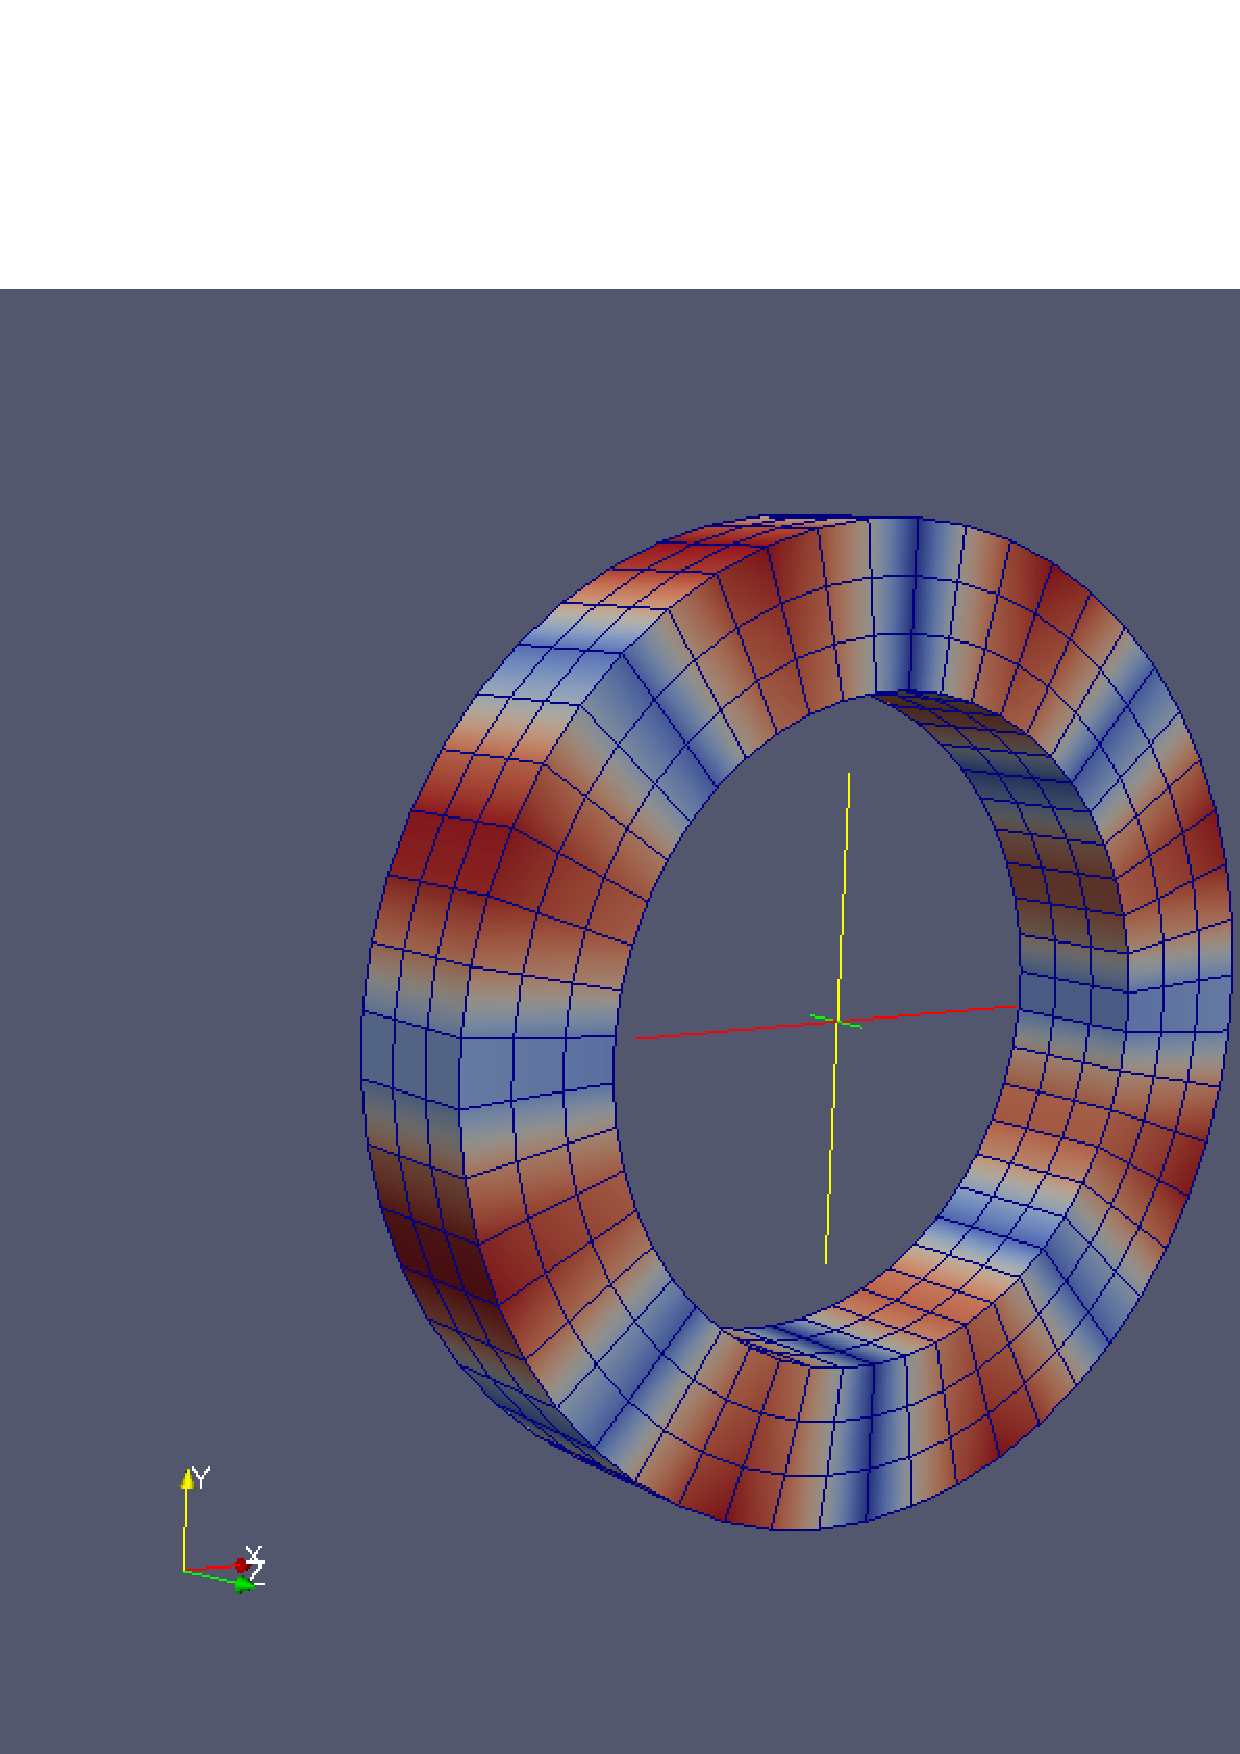
\includegraphics[width=80mm]{RingProjLieNo.pdf}}
    \subfigure[]{
      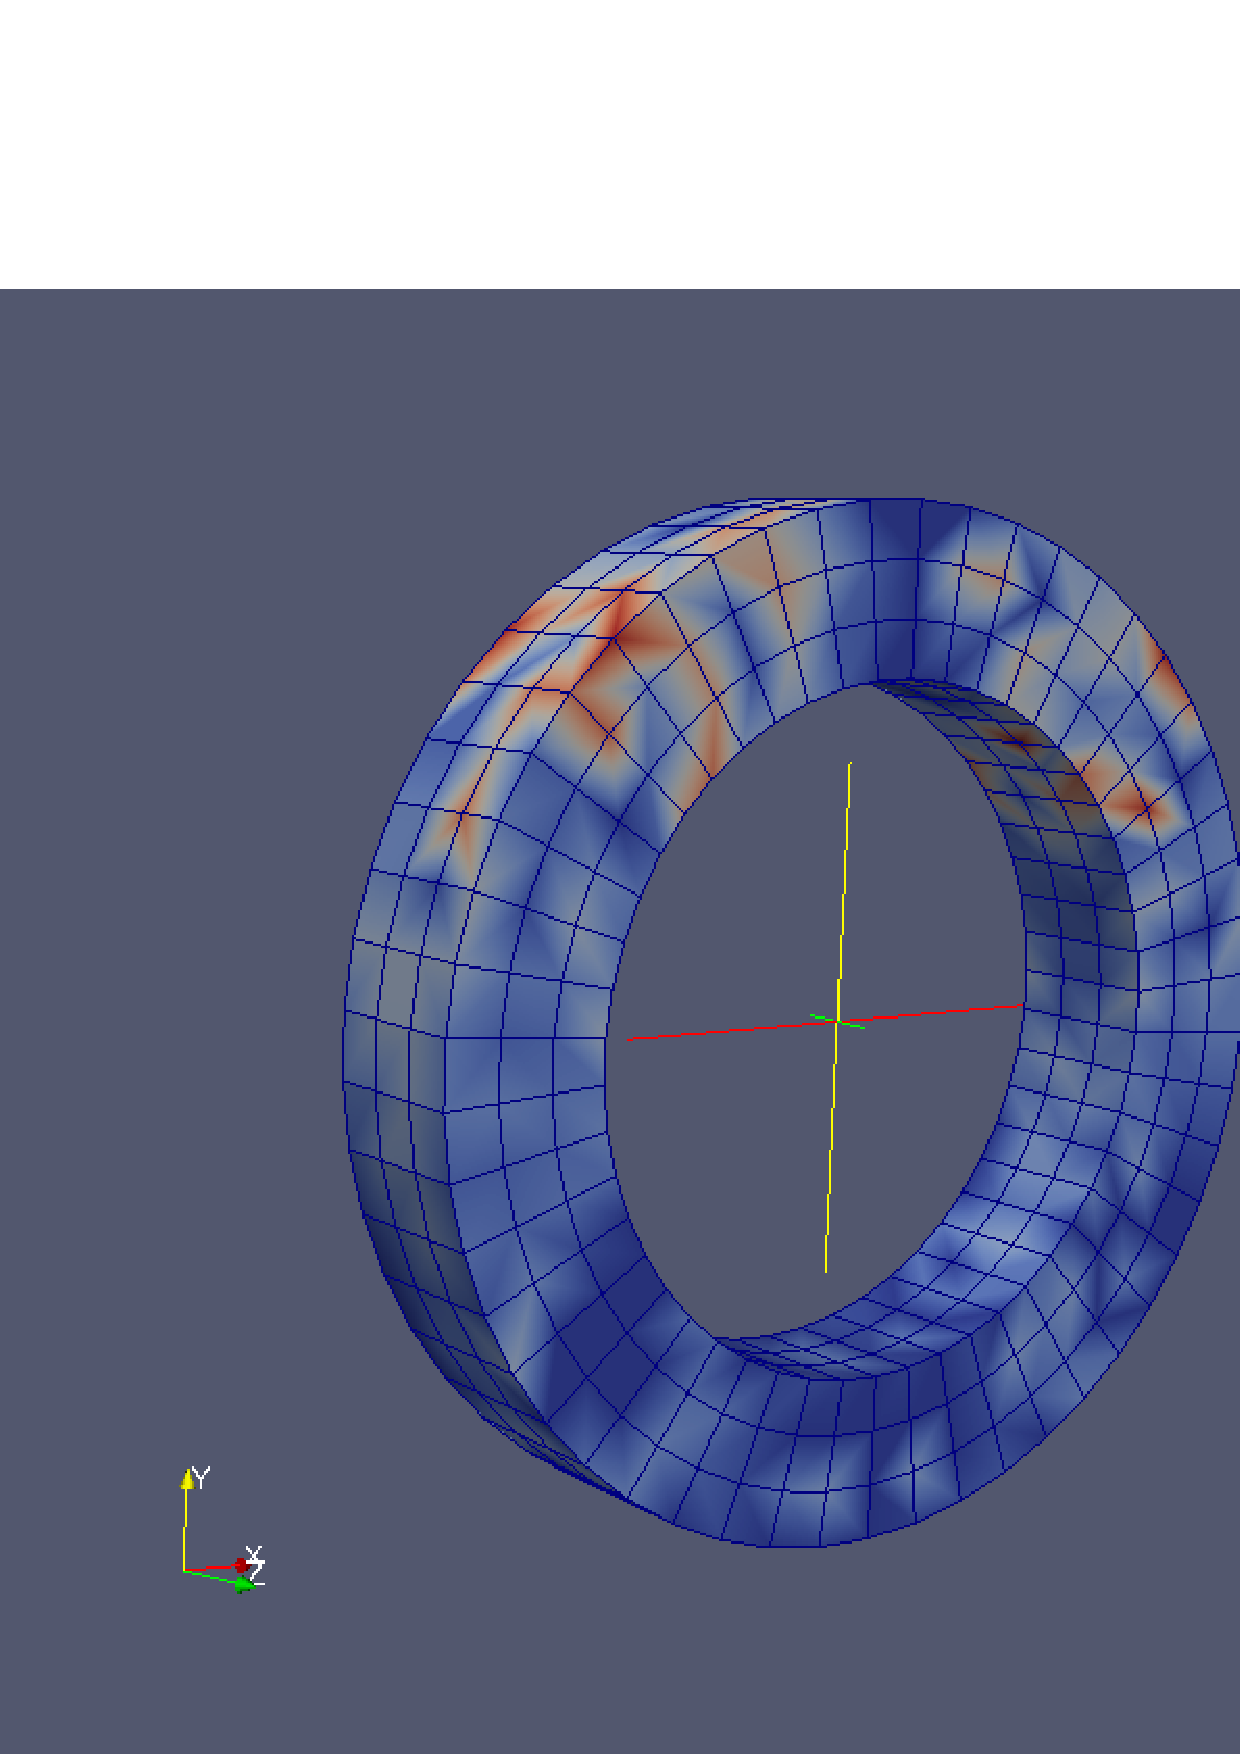
\includegraphics[width=80mm]{RingProjLieHALF.pdf}}
    \subfigure[]{
      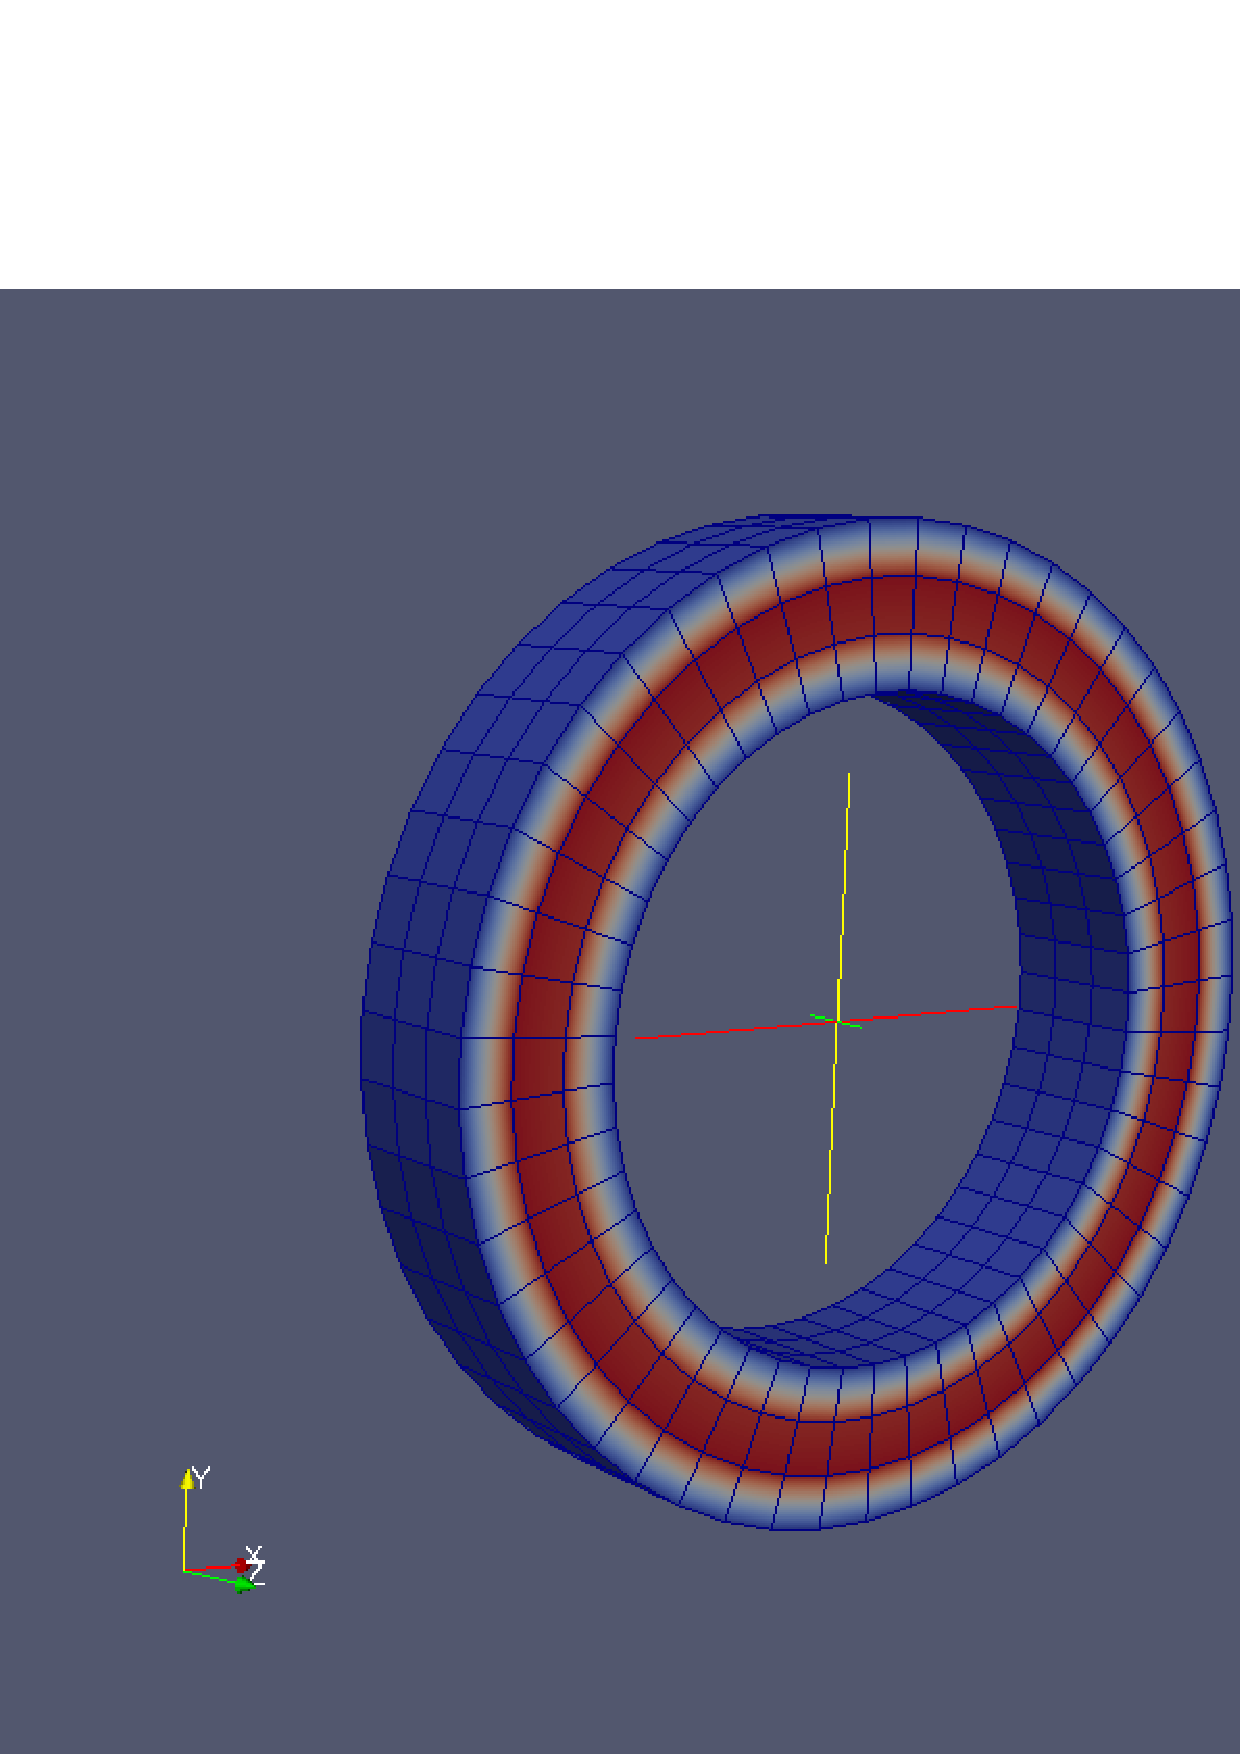
\includegraphics[width=80mm]{RingProjLieFULL.pdf}}
    \caption{Interpolation error \eqref{eq:Frobenius-norm-distribution}
      for different interpolation schemes: (a) direct interpolation of
      rotation and stretch; (b) Lie algebra interpolation of rotation
      and direct interpolation of stretch; (c) Lie algebra
      interpolation of rotation and stretch.}
    \label{fig:example-ring}
  \end{center}
\end{figure}

Next are the results of using Lie algebra interpolation for the rotation and
direct interpolation for the stretch, shown in Figure \ref{fig:example-ring}(b).
There is a significant improvement of accuracy when using this scheme, as the
maximum error $e_{\text{max}} = 1.2 \times 10^{-15}$ is reduced by $14$ orders
of magnitude.

Finally, Figure~\ref{fig:example-ring}(c) shows the results of applying Lie
algebra interpolation for both the rotation and the stretch. The maximum value
of the interpolation error now becomes $e_{\text{max}} = 0.018$, which falls in
between the values of the two cases discussed above. This is due to the fact
that the stretch given by \eqref{eq:polar-decomposition} varies linearly along
the $Y$ direction. Thus, the direct linear interpolation can reproduce the
stretch exactly, while the Lie algebra interpolation cannot. This example
demonstrates that the appropriate choice of interpolation scheme depends on the
nature of the field. Note that in general, however, the stretch is unlikely to
have this simple form and linear extrapolation may result in stretches that are
not positive definite.

\subsubsection{The Effect of Mesh Refinement}

We investigate the effect of mesh refinement on the overall accuracy of the
three interpolation schemes mentioned above. The error measure defined by the
norm \eqref{eq:norm} on the tensor field $\bA$ is evaluated numerically at a
variety of refinement levels, \emph{i.e.}
\begin{align}
  E_{\bA} & =
  \left(
    \int_{B} || \bA^{h}(\bX)- \bA(\bX) ||^2_{F} \, dV
  \right)^{\frac{1}{2}} \nonumber
  \\
  & \approx
  \left(
    \sum^{N_E}_{j=1}\sum^{N_G}_{i=1}
    || \lambda_{\alpha} (\bxi_{i}) \bA_{\alpha} - \bA(\bxi_{i}) ||^2_{F} \;
    w(\bxi_{i})  J(\bxi_{i})
  \right)^{\frac{1}{2}}
  \label{eq:Frobenius-norm-global}
\end{align}
where $\bA$ can be any of $\bF$, $\bR$ or $\bU$, $E_{\bA}$ is the error
corresponding to the interpolated tensor field $\bA$, $\bxi_i$ is the
integration point in the parametric domain, $w(\bxi_i)$ is the weight of
the Gauss quadrature, $J(\bxi_i)$ is the Jacobian determinant of the
isoparametric mapping, $N_G$ is the number of integration points per
element, and $N_E$ is the number of elements in the mesh.

Initially, the domain of size $L \times \frac{L}{16} \times \frac{L}{16}$ is
meshed by four elements along the $X$ (length) direction and one element along
the $Y$ (height) and $Z$ (width) directions. The aspect ratio of length divided
by height of all the elements is therefore $\frac{l}{h}=4$. Then, we refine the
mesh by increasing the number of elements in both the $X$ and $Y$ directions,
but maintain the number of elements along the $Z$ direction equal to one. In
each refined mesh, the aspect ratio remains constant and equal to four for all
elements.

\begin{figure}[htbp]
  \begin{center}
    \unitlength=1.0mm
    \subfigure[]{
      \includegraphics[width=80mm]{RefinementF.pdf}}
    \subfigure[]{
      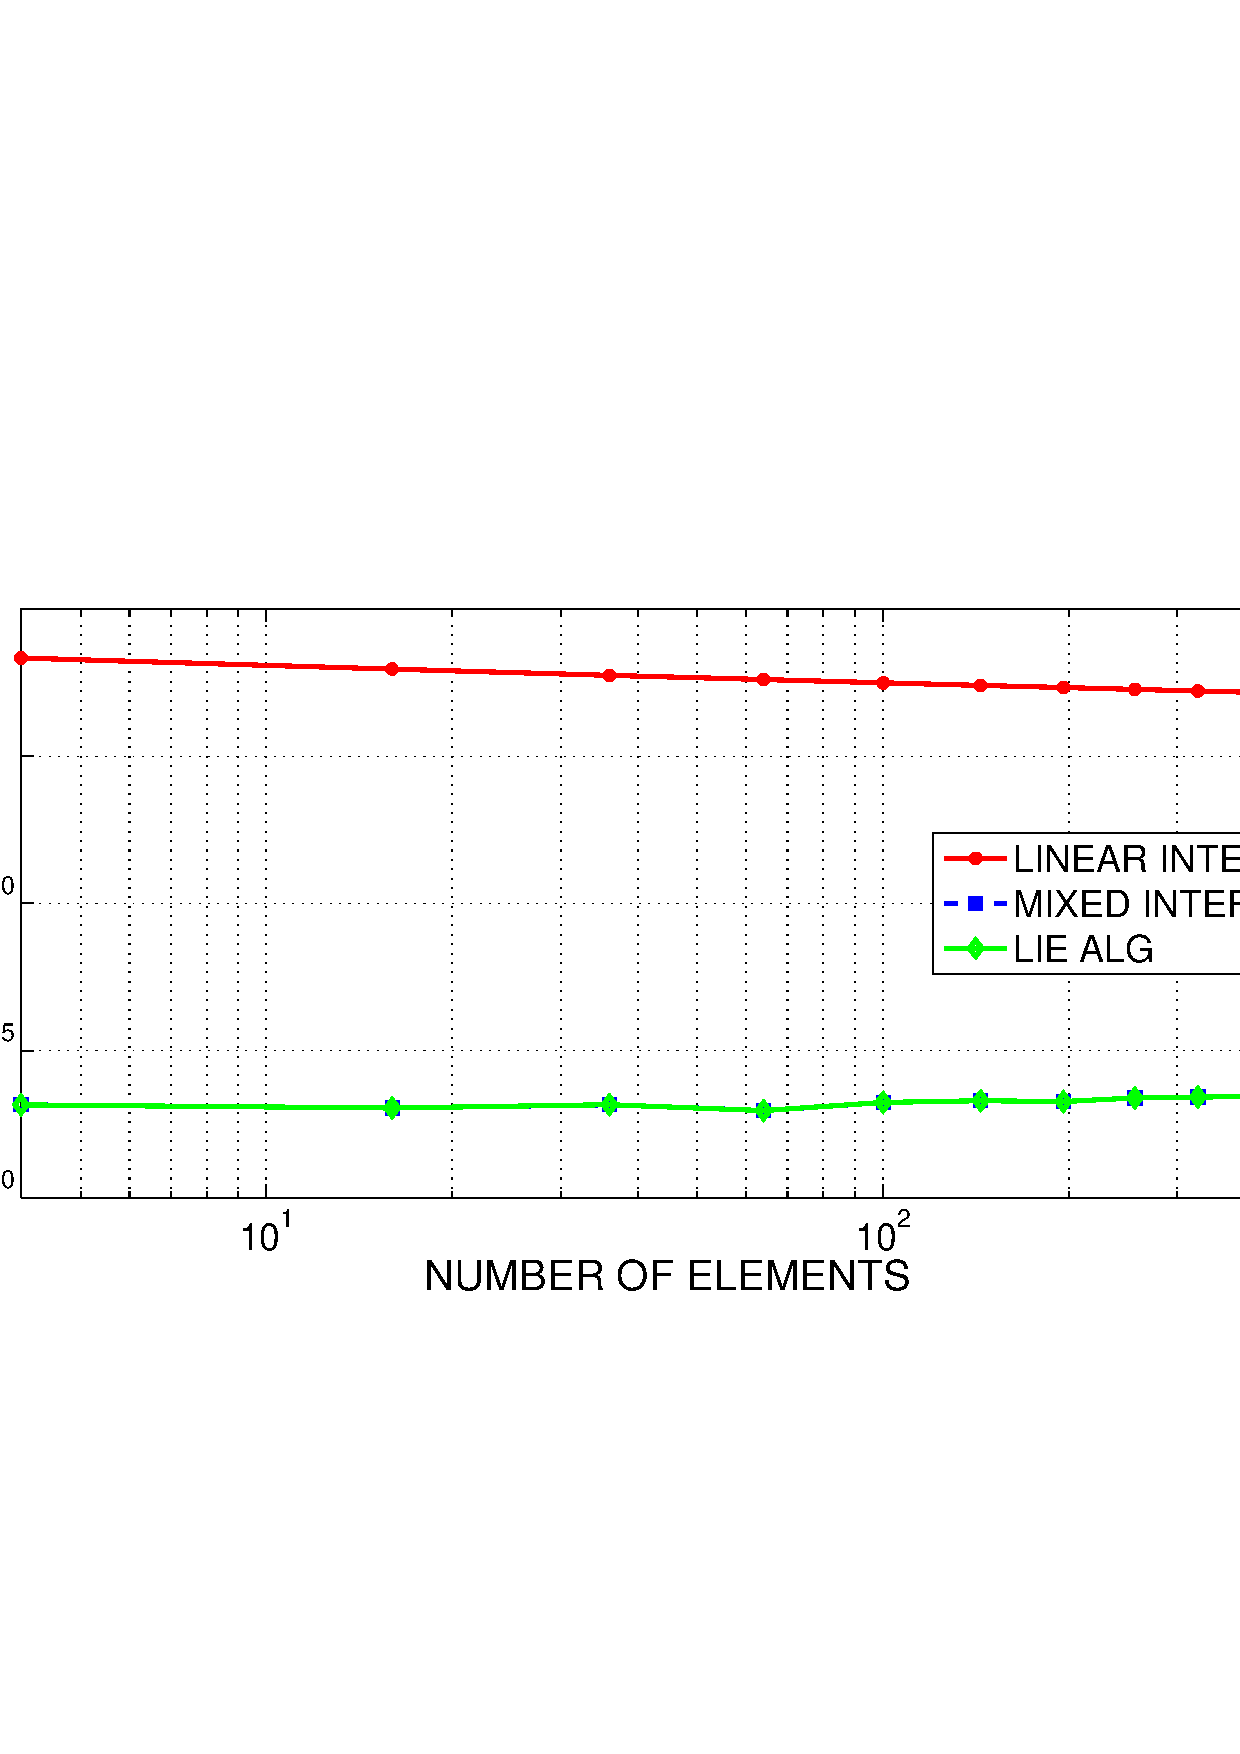
\includegraphics[width=80mm]{RefinementR.pdf}}
    \subfigure[]{
      \includegraphics[width=80mm]{RefinementU.pdf}}
    \caption{Convergence plots for the ring bending problem: error in
      (a) deformation gradient, (b) rotation and (c) right stretch.}
    \label{fig:ring-refinement}
  \end{center}
\end{figure}

Figures~\ref{fig:ring-refinement}(a)-(c) show the convergence curves
for the three interpolation schemes. The curves correspond to: direct
interpolation for both rotation and stretch (red), Lie algebra
interpolation for the rotation and direct interpolation for the
stretch (blue), and Lie algebra interpolation for both the rotation
and the stretch (green).

The behavior exhibited by the curves reflects the ability of each interpolation
scheme to reproduce the corresponding exact field. For the ring configuration,
the logarithm of the rotation can be readily computed using
\eqref{eq:log-rotation}, while the logarithm of the stretch is trivial to
compute in the canonical basis $\be_i$. Thus, from
\eqref{eq:polar-decomposition} we obtain
\begin{equation}
  [\log \bR(X)]_{\be_i} =
  \begin{pmatrix}
    0 & - \frac{X}{R} & 0
    \\[0.3em]
    \frac{X}{R} & 0  & 0
    \\[0.3em]
    0 & 0 & 0
  \end{pmatrix},
  \quad
  [\log \bS(Y)]_{\be_i} =
  \begin{pmatrix}
    \log (\frac{R-Y}{R})  & 0 & 0
    \\[0.3em]
    0 & 0 & 0
    \\[0.3em]
    0 & 0 & 0
  \end{pmatrix}.
  \label{eq:log-polar-decomposition} 
\end{equation}

It is immediately apparent from \eqref{eq:polar-decomposition} and
\eqref{eq:log-polar-decomposition} that, as the logarithm of the
rotation and the stretch are both linear with respect to the reference
coordinates, the best scheme for this case is to use Lie algebra
interpolation for the rotation and direct interpolation for the
stretch. This is clearly confirmed by Figures
\ref{fig:ring-refinement}(a)-(c). The interpolation error of the
deformation gradient is shown in Figure~\ref{fig:ring-refinement}(a),
which shows linear convergence for direct interpolation, linear
convergence for Lie algebra interpolation, and exact representation,
up to machine precision, for mixed interpolation. Convergence on the
rotation is examined further in Figure~\ref{fig:ring-refinement}(b),
in which both schemes that use Lie algebra interpolation for the
rotation are exact, up to machine precision. Conversely, convergence
for the stretch is exact up to machine precision when using direct
interpolation, as shown in Figure~\ref{fig:ring-refinement}(c).

Note that Lie algebra interpolation for both rotation and stretch has
less error than direct interpolation for both rotation and stretch,
despite the fact that the stretch is linear with respect to the
reference coordinates.

\subsubsection{Comparison with Other Recovery Schemes}
\label{sec:recovery-schemes}

We now compare the performance of the variational transfer operator with respect
to other customary transfer schemes. To this end, the values of the exact
deformation gradient \eqref{eq:deformation-gradient} are computed at the
integration points of a $16$-element coarse mesh and then transferred to the
nodes by means of various recovery methods. The assumption is that once nodal
values are obtained, the element interpolation functions are used to extend the
field over the entire domain for the purpose of mapping it to a different mesh.
The schemes are summarized as follows:
\begin{enumerate}
  \item Direct averaging that employs a searching scheme to determine
  the closest integration point to a node in each element. The value
  of the closest integration point is then assigned to the node. If
  the same node is shared by more than one element, then the
  integration point values are averaged among the elements attached to
  that node.
  \item Extrapolation. Additional interpolation functions are
  established using the integration points as local nodes, then the
  fields at the integration points are extrapolated to the actual
  nodes of each finite element. The nodal values are then averaged as
  in the previous scheme.
  \item Variational transfer operator with polar decomposition
  and direct interpolation.
  \item Variational transfer operator with no polar decomposition and
    direct interpolation.
  \item Variational transfer operator with polar decomposition, Lie
    algebra interpolation for the rotation and direct interpolation
    for the stretch.
  \item Variational transfer operator with polar decomposition and Lie
    algebra interpolation for both the rotation and stretch.
\end{enumerate}

The minimum and maximum error \eqref{eq:Frobenius-norm-distribution} at the
nodes as well as the global error \eqref{eq:Frobenius-norm-global} of the six
recovery procedures are compared in Table \ref{tab:ring-error-comparison}.

\begin{table}[htbp]
  \begin{center}
    \begin{tabular}{ l l l l }
      \toprule      
      \multirow{2}{*}{Method}
      &
      \multicolumn{2}{c}{$e(\bX_{\alpha})$}
      & 
      \multicolumn{1}{c}{\multirow{2}{*}{$E_{F}$}}
      \\
      &
      \multicolumn{1}{c}{min}
      &
      \multicolumn{1}{c}{max}
      &
      \\
      \hline
      Direct Averaging
      &
      $6.34 \times 10^{-2}$
      &
      $1.41 \times 10^{-1}$
      & 
      $8.70 \times 10^{-3}$
      \\
      Extrapolation   
      &
      $6.62 \times 10^{-2}$
      &
      $6.96 \times 10^{-1}$
      &
      $5.08 \times 10^{-2}$
      \\
      Variational (polar, direct)
      &
      $1.68 \times 10^{-2}$
      &
      $1.99 \times 10^{-2}$
      & 
      $2.01 \times 10^{-4}$
      \\
      Variational (no polar, direct)
      &
      $1.68 \times 10^{-2}$
      &
      $1.99 \times 10^{-2}$
      & 
      $2.01 \times 10^{-4}$
      \\
      Variational (polar, mixed)  
      &
      $5.38 \times 10^{-16}$
      &
      $2.45 \times 10^{-13}$
      & 
      $3.30 \times 10^{-16}$
      \\
      Variational (polar, both Lie)  
      &
      $7.80 \times 10^{-3}$
      &
      $8.70 \times 10^{-3}$
      & 
      $3.35 \times 10^{-16}$
      \\
      \bottomrule
    \end{tabular}
    \caption{Minimum and maximum error
      \eqref{eq:Frobenius-norm-distribution} at the nodes and global error
      \eqref{eq:Frobenius-norm-global} of various recovery methods for
      the bending ring problem.}
    \label{tab:ring-error-comparison}
  \end{center}
\end{table}

The table shows that the four variational projection cases result in less error
than both the direct averaging and extrapolation methods, regardless of whether
Lie algebra interpolation is employed. This is consistent with the proposition
in section~\ref{sec:FE-formulation} in which the variational operator is proved
to minimize the $L_2$ norm. Furthermore, the global error measured by $E_{F}$ is
reduced by a minimum of $12$ orders of magnitude when the interpolation for the
rotation is conducted in $so(3)$ instead of $SO(3)$.

Even though the local error measure at the nodes $e(\bX_{\alpha})$ is
lower in the variational approach with mixed interpolation than in the
variational approach with full Lie algebra interpolation, the
reduction in global error $E_{F}$ is within the same order. This is
explained by recalling that the values of the field at the integration
points are computed using the exact expression
\eqref{eq:deformation-gradient}. When projecting to the nodes using
Lie algebra interpolation, some error is introduced into the stretch,
as discussed before. This error is manifested in the values of the
nodal local error $e(\bX_{\alpha})$. In the computation of the global
error $E_F$, however, the nodal quantities are used to compute new
values at the integration points. These new integration point values
are very close to the original ones computed using the exact
expression, hence the low values for the global error.


\subsection{Elastic-Plastic Upsetting of an Axisymmetric Billet}

This example demonstrates the ability of the variational transfer operator to
maintain internal variables in their admissible space. The variational
projection operator and the Lie algebra interpolation techniques are integrated
into a unified framework. The simulation is a severe deformation test problem
proposed by \citet{Krieg.Krieg:1977} and further examined by
\citet{Taylor.Becker:1983} and \citet{Simo.Hughes:1998}. For completeness, we
briefly review the statement of the problem below.

Consider a cylindrical billet with initial radius $r = 10\text{mm}$
and initial height $h = 30\text{mm}$. Due to radial symmetry, only
$\frac{1}{8}$ of the domain is included in the calculation. The top of
the cylinder is fixed by a roller such that it does not move
vertically but is free to expand horizontally. The bottom of the
cylinder is fixed horizontally, and a prescribed vertical displacement
is applied to it.  The constitutive response of the specimen is
simulated via a $J_2$ elasto-plastic model with linear isotropic
hardening. The material parameters used for this calculation are those
listed in \citet{Taylor.Becker:1983} and \citet{Simo.Hughes:1998} (see
Table~\ref{tab:upset-billet}).

\begin{table}[htbp]
  \begin{center}
    \begin{tabular}{ l l }
      \toprule      
      Young's modulus
      &
      $E = 1000$MPa
      \\
      Poisson's ratio
      &
      $\nu = 0.3$
      \\
      Yield stress  
      &
      $\sigma_{y} = 1.00$MPa
      \\
      Hardening modulus   
      &
      $H=3.0$MPa
      \\
      \bottomrule
    \end{tabular}
    \caption{Material parameters for cylindrical billet.}
    \label{tab:upset-billet}
  \end{center}
\end{table}

Four finite element simulations are performed using Sandia's Laboratory for
Computational Mechanics (LCM\texttrademark) code \citep{lcm}. To preserve the
radial symmetry of the cylinder, hexahedral meshes are generated via a radial
meshing algorithm in Sandia's \textsc{cubit} mesh generation software in such a
manner that node distribution is unbiased along the radial direction
\citep{cubit}. $8$-node and $27$-node Lagrange hexahedral elements are both used
on two meshes consisting of $693$ and $2175$ elements. The final configuration
in all four simulations is attained using adaptive loading steps.
Figure~\ref{fig:load-deflection} shows the resulting load-deflection curves.
These results are in good agreement with \citet{Krieg.Krieg:1977},
\citet{Taylor.Becker:1983} and \citet{Simo.Hughes:1998}.

\begin{figure}[htbp]
  \begin{center}
    \unitlength=1.0mm
      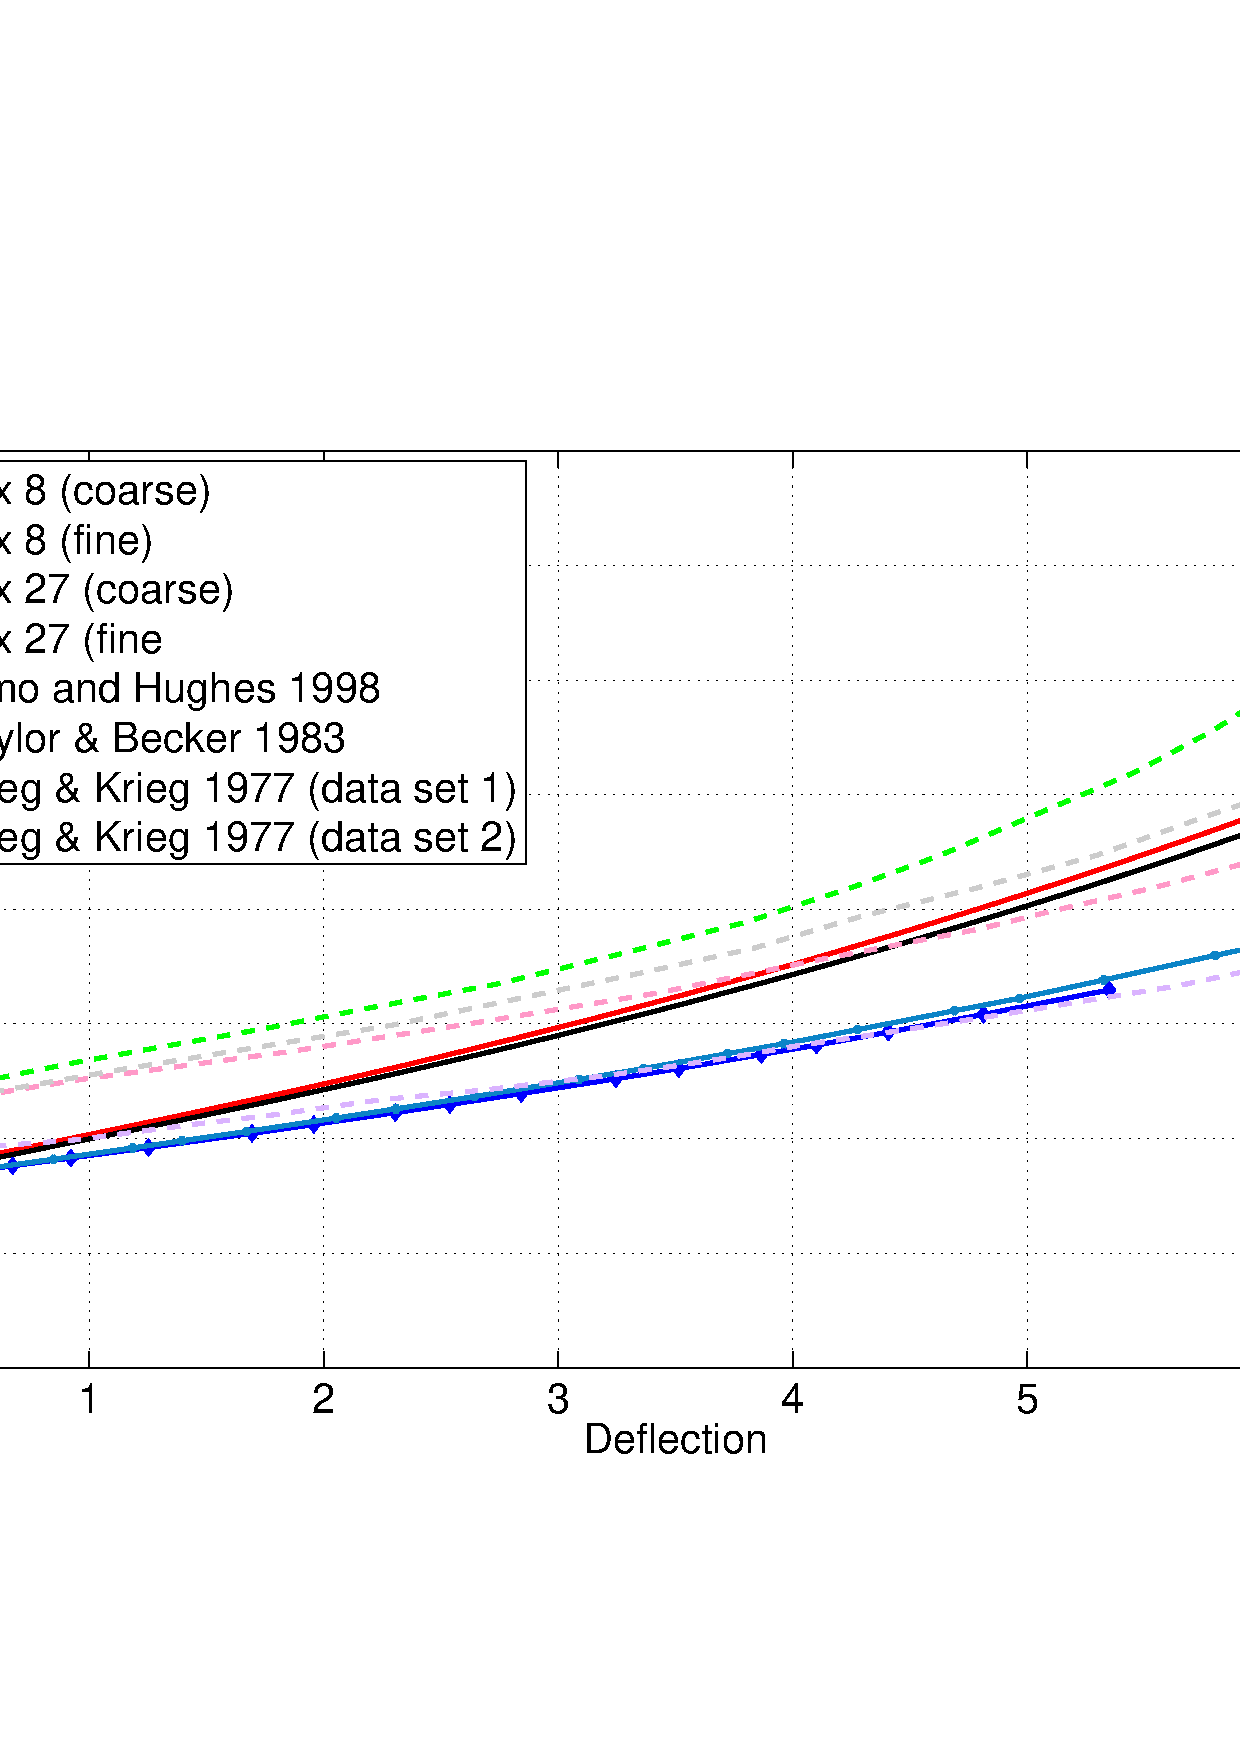
\includegraphics[width=160mm]{Load_Deflection.pdf}
      \caption{Load-deflection curve of the elastic-plastic upsetting
        of an axisymmetric billet. }
    \label{fig:load-deflection}
  \end{center}
\end{figure}

\subsubsection{Admissible Range of Isochoric Plastic Response}

The simulations are advanced until the billet has reached an upsetting of
$53\%$, wherein the plastic part of the deformation gradient $\bF^{p} =
(\bF^{e})^{-1} \bF$ computed at each integration point is extended to the entire
domain by means of the variational transfer operator.
Figure~\ref{fig:billet-no-Lie} shows the extended $\bF^{p}$ fields of the two
$8$-node element meshes using direct interpolation. The color in the figure
represents the determinant of $\bF^{p}$.

The flow rule for $J_2$ plasticity is
\begin{equation}
  \dot{\bF^p} {\bF^p}^{-1} = \dot{\varepsilon}^p \bM \in sl(3),
  \label{J2-flow-rule}
\end{equation}
in which $\dot{\varepsilon}^p$ is the equivalent plastic strain rate
and $\bM$ is the direction of plastic flow, with $\tr \bM = 0$ and
$\bM:\bM = \frac{3}{2}$ \citep{Ortiz.Stainier:1999}. This flow rule is
a kinetic equation of the form \eqref{eq:time-derivative-general}, and
therefore it is required that the plastic part of the deformation
gradient be isochoric, or equivalently that its determinant be equal
to one, \emph{i.e.} $\bF^p \in SL(3)$ as stated in
Table~\ref{tab:examples-evolution}.

Our simulation results indicate, however, that this is not necessarily the case
when the $L_2$ projection is performed without transforming $\bF^{p}$ to its
corresponding Lie algebra for interpolation, thus violating one of the
fundamental assumptions of $J_2$ plasticity. By using direct interpolation for
$\bF^p$, spurious volumetric plastic deformations are introduced into the
extended field. This is evident in Figure~\ref{fig:billet-no-Lie}, in which the
determinant of the extended plastic part of the deformation gradient is in the
range $\det \bF^p \in [0.83, 1.24]$ for the coarse mesh, and $\det \bF^p \in
[0.64, 1.40]$ for the fine mesh.

This severe error occurs when the mesh is subjected to a significant amount of
distortion at the edge of the bottom face, as shown in Figure
\ref{fig:billet-no-Lie}(a). The spurious plastic volumetric strain is not
eliminated through refinement, as the significant distortion of the finite
element mesh is present regardless of mesh size.

\begin{figure}[htbp]
  \begin{center}
    \unitlength=1.0mm
    \subfigure[]{
      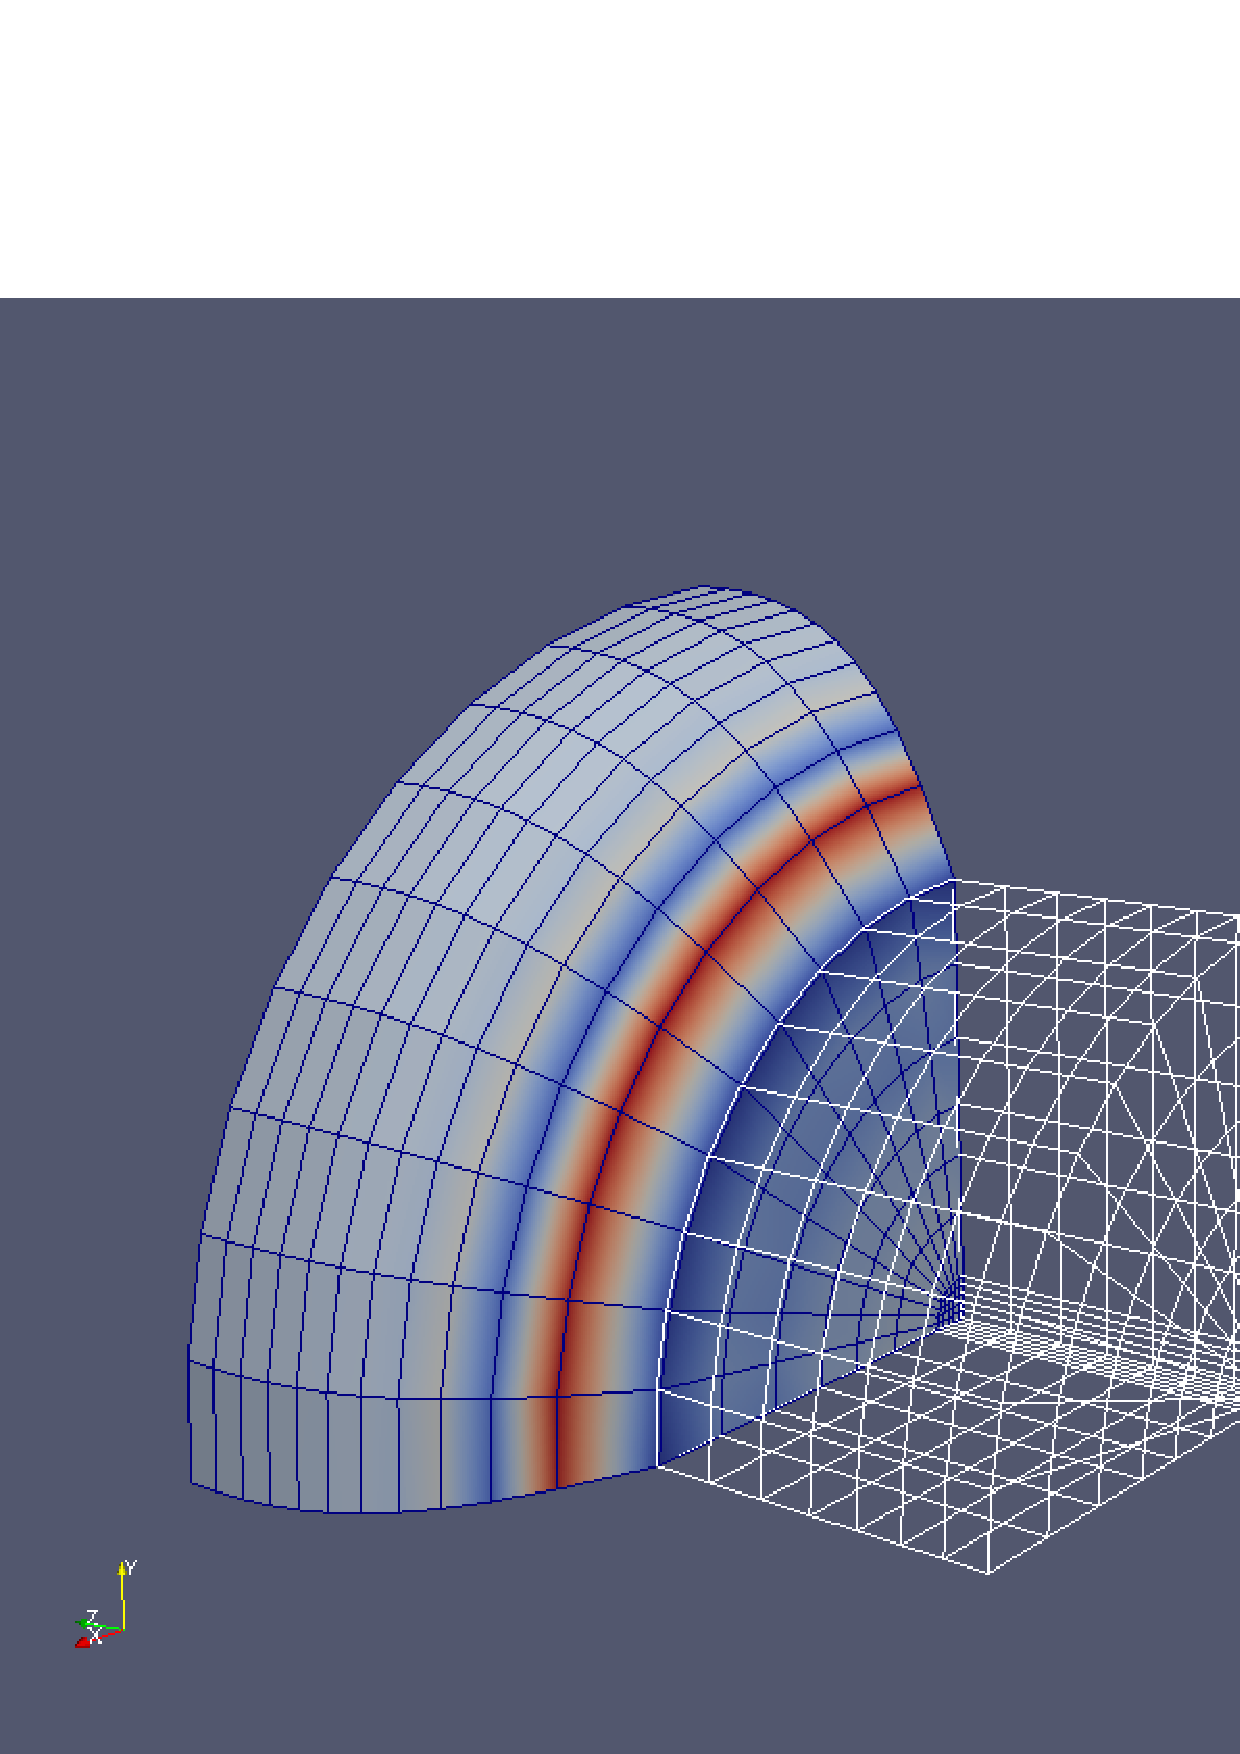
\includegraphics[width=80mm]{HEX8medium_DIRECT_woLie.pdf}}
    \subfigure[]{
      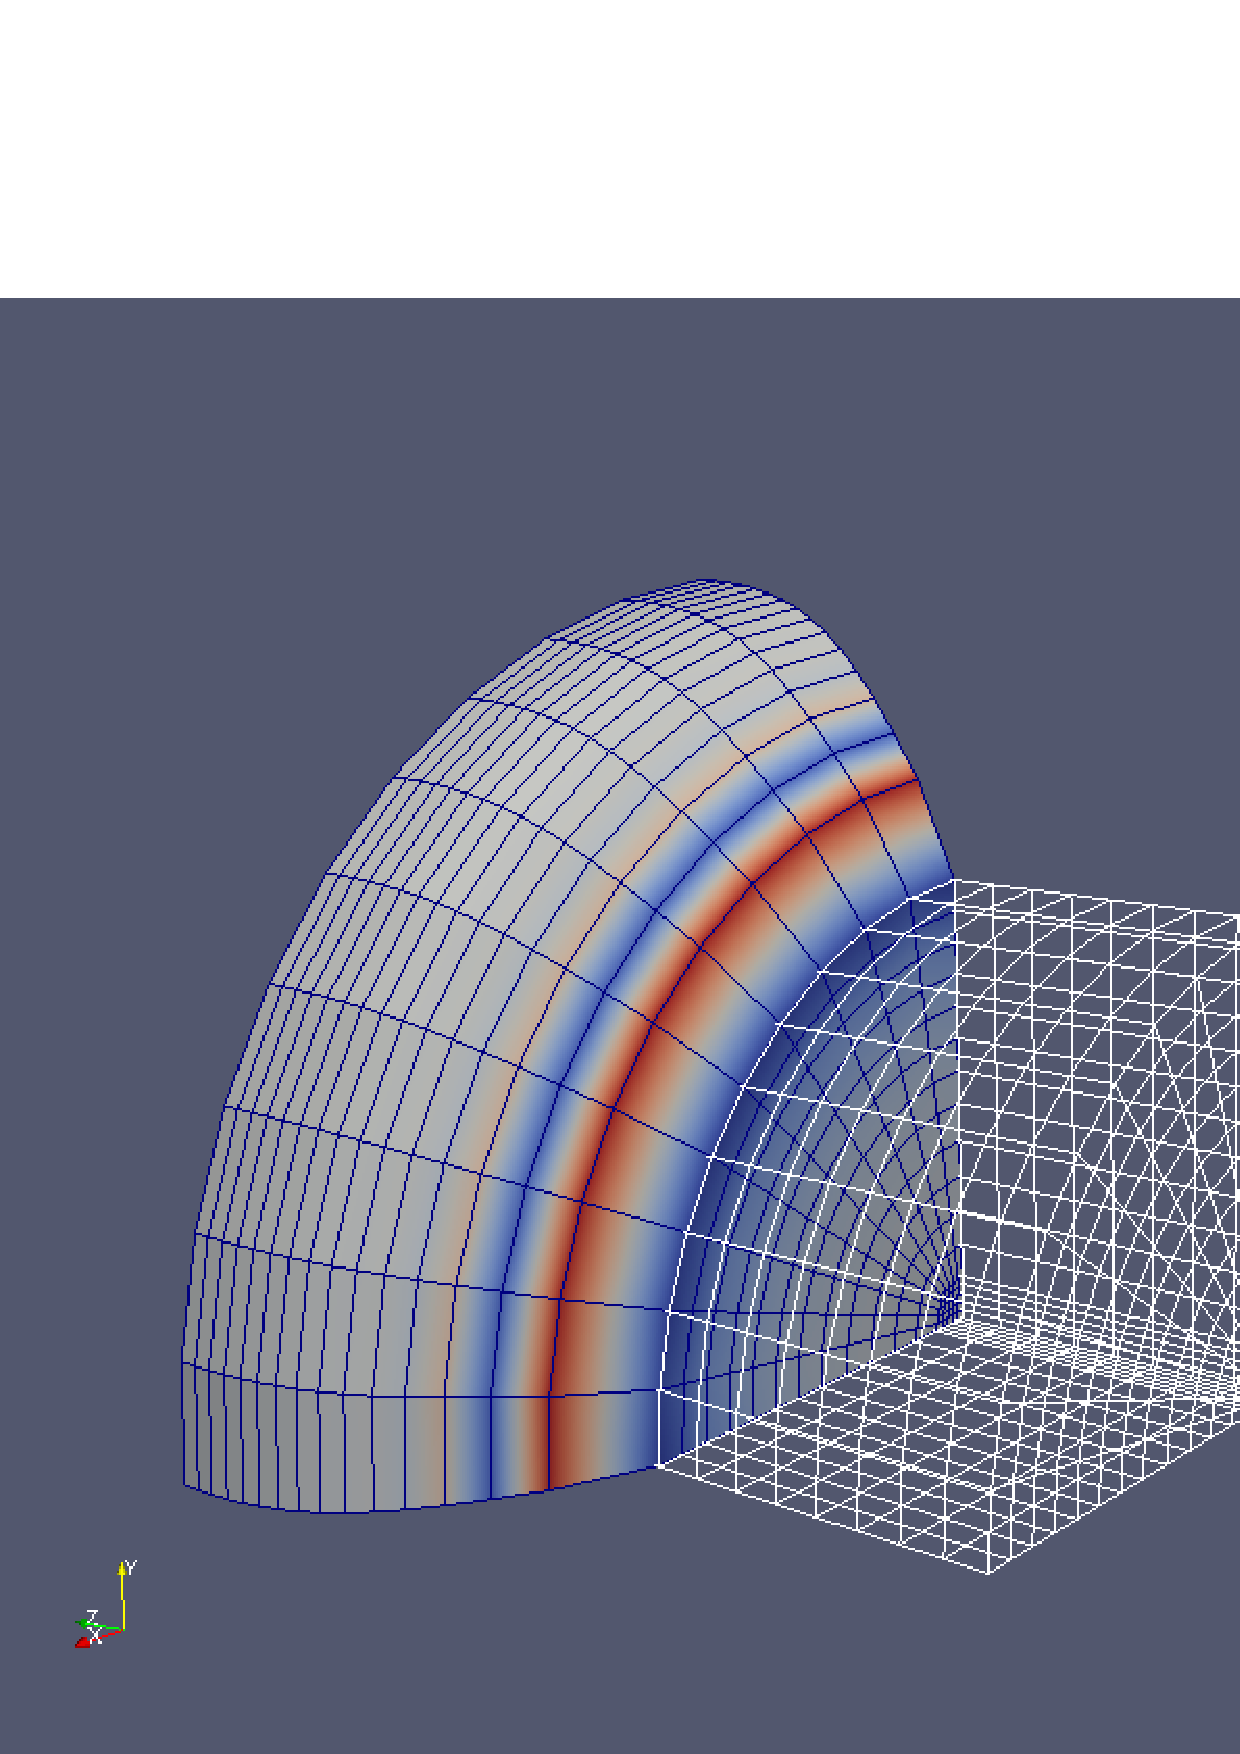
\includegraphics[width=80mm]{HEX8fine_DIRECT_woLie.pdf}}
    \caption{Plastic part of the deformation gradient by  direct interpolation:
    (a) $693$-element mesh and (b) $2175$-element mesh.}
    \label{fig:billet-no-Lie}
  \end{center}
\end{figure}

If the projection of the plastic part of the deformation gradient $\bF^{p}$ is
conducted through Lie algebra interpolation, then it remains isochoric as
illustrated in Figure~\ref{fig:billet-Lie}. This projection is obtained by first
decomposing $\bF^{p}$ into rotation and right stretch tensors via the singular
value decomposition as described in \eqref{eq:SVD-polar-1} to
\eqref{eq:SVD-polar-4}. Then, the rotation tensor is mapped from $SO(3)$ into
$so(3)$ using the logarithmic map \eqref{eq:log-rotation} and the stretch is
mapped from $GL^{+}(3)$ to $gl(3)$ by means of the logarithmic map
\eqref{eq:log-stretch}.

By applying the projection \eqref{eq:projection-z} on $so(3)$ and $gl(3)$ where
the addition operation is valid, the projected field is guaranteed to remain in
the admissible space. The projected fields are then transformed from their Lie
algebras $so(3)$ and $gl(3)$ back to their Lie groups $SO(3)$ and $GL(3)$. The
extended plastic part of the deformation gradient is then recovered by $\bF =
\bR \bS$ at any point of the finite element mesh. The results obtained from this
calculation show that the determinant of the plastic part of the deformation
gradient is equal to one (up to machine precision) everywhere in the domain. No
spurious dilation or contraction is introduced due to the projection from
integration points to nodes. This in effect prevents the injection of
non-physical data into the simulation when remeshing or post-processing take
place. Figure \ref{fig:billet-Lie} shows that the isochoric constraint is
preserved for both the coarse and the fine meshes.

\begin{figure}[htbp]
  \begin{center}
    \unitlength=1.0mm
    \subfigure[]{
      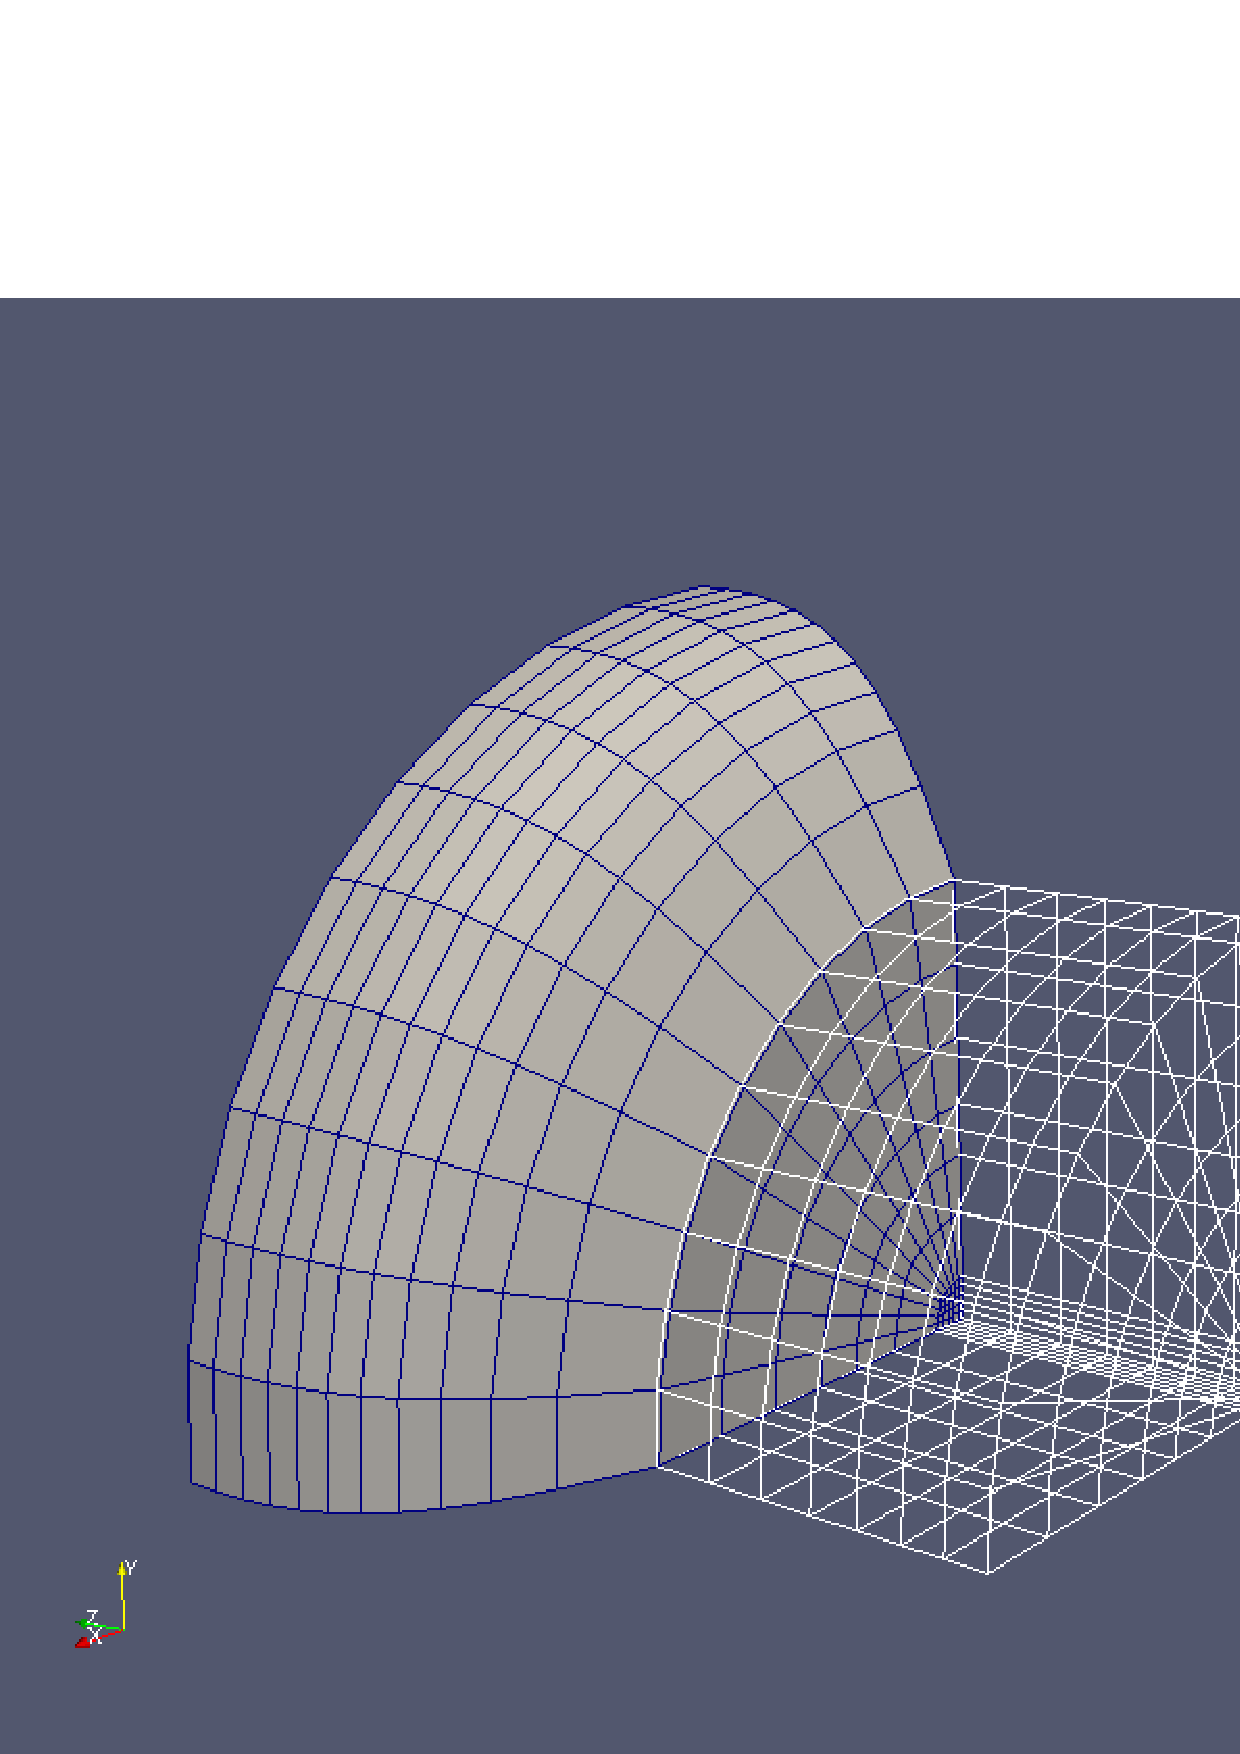
\includegraphics[width=80mm]{HEX8medium_DIRECT_wLie.pdf}}
    \subfigure[]{
      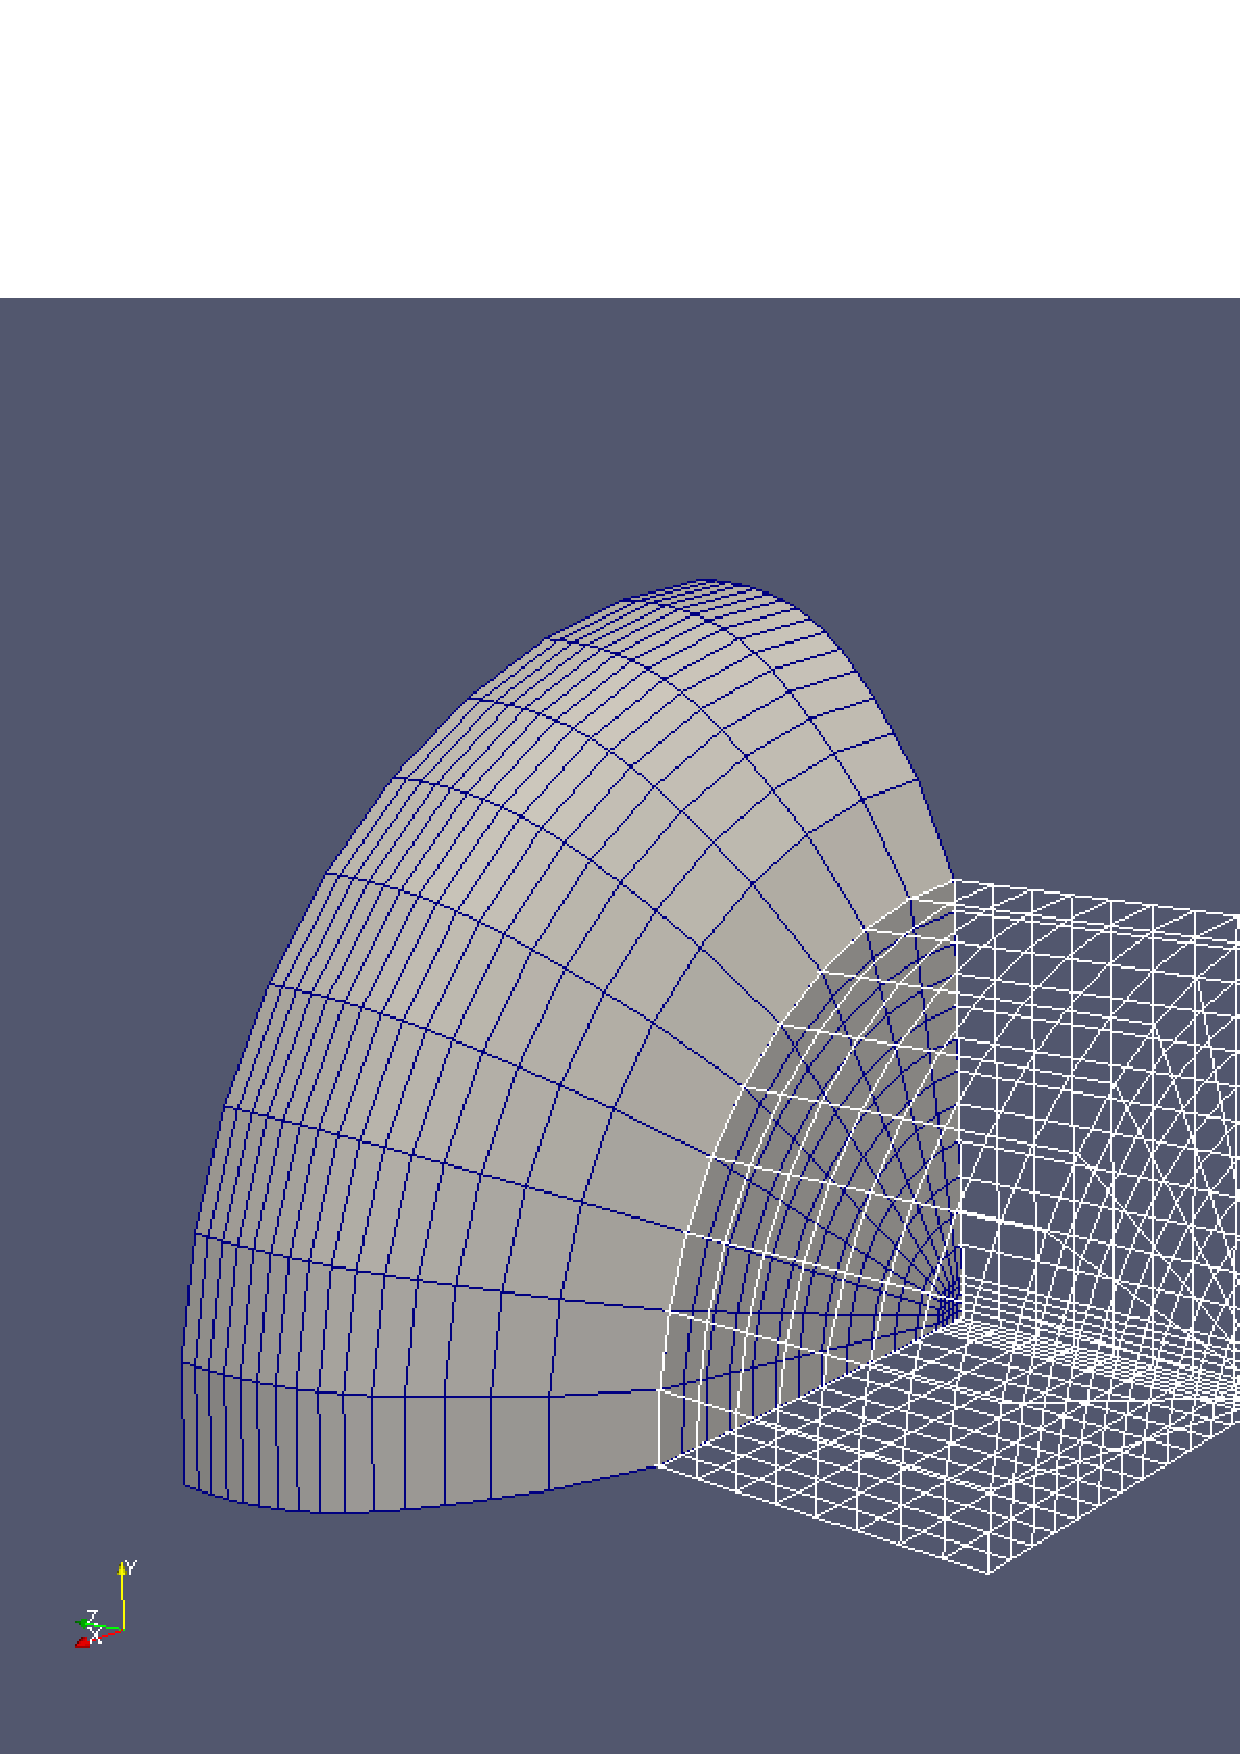
\includegraphics[width=80mm]{HEX8fine_DIRECT_wLie.pdf}}
    \caption{Plastic part of the deformation gradient by Lie group and Lie
    algebra interpolation: (a) $693$-element mesh and (b) $2175$-element mesh.}
    \label{fig:billet-Lie}
  \end{center}
\end{figure}

\subsubsection{Comparisons with Other Internal Variable Recovery Schemes}

We compare the performance of the same set of internal variable recovery schemes
discussed in Section~\ref{sec:recovery-schemes} but now using the upsetting
billet example. The plastic part of the deformation gradient $\bF^{p}$ at the
integration points of the coarse mesh is first projected to the nodes. Using
these nodal values and the element interpolation functions, the field is
extended over the entire domain, and this extended field is used to compute the
global error as defined in \eqref{eq:Frobenius-norm-global}.
Table \ref{tab:billet-error-comparison} shows the results. Among the six
internal variable recovery schemes, only the ones using Lie algebras are able to
preserve the isochoric constraint of the $J_2$ plasticity model. As before, in
the computation of the global error $E_F$, the nodal quantities are used to
compute new values at the integration points. The new integration point values
are very close to the original ones, resulting the low values for the global
error.

Despite low values of the global error, it is clear that using direct
interpolation leads to large errors in the range of $\det \bF^p$, and therefore
any mapping of $\bF^p$ to a new mesh that relies in direct interpolation will
introduce large errors into the field. Only the use of Lie algebra interpolation
guarantees that the isochoric constraint will be preserved when mapping the
field to a new mesh.
 
\begin{table}[htbp]
  \begin{center}
    \begin{tabular}{ l l l l }
      \toprule
      \multirow{2}{*}{Method}
      &
      \multicolumn{2}{c}{$\det \bF^{p}$}
      & 
      \multicolumn{1}{c}{\multirow{2}{*}{$E_{F}$}}
      \\
      &
      \multicolumn{1}{c}{min}
      &
      \multicolumn{1}{c}{max}
      &
      \\
      \hline
      Direct Averaging
      &
      $1.00$
      & 
      $1.24$
      & 
      $9.35 \times 10^{-9}$
      \\
      Extrapolation   
      &
      $0.95$
      &
      $1.10$
      &
      $1.56 \times 10^{-8}$
      \\
      Variational (polar, direct)
      &
      $0.89$
      & 
      $1.10$
      & 
      $7.36 \times 10^{-9}$
      \\
      Variational (no polar, direct)
      &
      $0.83$
      & 
      $1.24$
      & 
      $7.40 \times 10^{-9}$
      \\
      Variational (polar, mixed)  
      &
      $1^\dagger$
      & 
      $1^\dagger$
      & 
      $7.37 \times 10^{-9}$
      \\
      Variational (polar, both Lie)  
      &
      $1^\dagger$
      & 
      $1^\dagger$
      & 
      $7.07 \times 10^{-9}$
      \\
      \bottomrule
    \end{tabular}
    \caption{Comparison of various internal variable recovery methods
      for the upsetting billet problem. $^\dagger$ Up to machine precision.}
    \label{tab:billet-error-comparison}
  \end{center}
\end{table}

\section{Conclusion}

The proposed transfer operator is composed of two parts: 1) the variational
$L_2$ projection that minimizes the error; 2) the mapping of fields to Lie
algebras for interpolation and mapping back to Lie groups.

We prove that the $L_2$ projection minimizes the error and that using Lie
algebras many of the common tensor fields can be interpolated while remaining in
their admissible spaces.

The numerical examples show the effect of using different schemes to project
fields from integration points to nodes in order to extend the field over the
entire domain of a finite element mesh. In turn, this extended field can mapped
to a different finite element mesh of the same domain. It is shown in the
numerical examples that the $L_2$ projection minimizes the error.
It is also shown that using direct interpolation leads to severe error when the
fields have constraints, such as the isochoric condition for $J_2$ plasticity.
The use of Lie algebras for interpolation avoids this situation altogether.

The computation of the logarithmic map leads to complex arithmetic for tensors
with negative eigenvalues. The proposed technique of using the singular value
decomposition to compute the polar decomposition, and then apply the logarithmic
map separately for the rotational and strech components of a tensor field proves
convenient to bypass complex arithmetic.

We conclude that the use of these techniques provide a powerful method for
extending fields of internal variables from integration points to the entire
domain, which in turn serves the purpose of mapping them to a different
discretization.

\section{Acknowledgments}

Support for this work was received through the Advanced Simulation and Computing
(ASC) Program at Sandia National Laboratories. Sandia is a multi-program
laboratory operated by Sandia Corporation, a Lockheed-Martin Company, for the
United States Department of Energy's National Nuclear Security Administration
under contract DE-AC04-94AL85000.

\bibliographystyle{plainnat}
\bibliography{tomiv}

\end{document}
